%\chapter{Reasoning Models}
\chapter{大语言模型中的多步推理}\label{chap:reasoning}


\begin{learningbox}
在本章中，你将学习语言模型如何通过{\em 多步推理}解决更复杂的问题。
具体来说，你将能够：
\begin{itemize}[leftmargin=*, nosep]
    \item 描述{\em 思维链}这一概念：我们如何用上下文学习引导大语言模型在回答查询时采取中间步骤，从而对更复杂的查询给出更好的回答。
    \item 描述推理方法如何极大地提升了 LLM 的{\em 能力}，以及为什么这种能力对智能体大语言模型在现实世界中真实地行动至关重要。
    \item 写出你的第一个{\em 智能体运行框架}：一个小算法，用不同的提示词调用 LLM。智能体运行框架负责管理提示词以及 LLM 的回复。
    \item 解释{\em 自我反思}：运行框架可以让 LLM 扮演不同角色，例如{\em 评估}一个答案，或{\em 生成}子问题。LLM 通过反思来改进自己的答案。
    \item 理解{\em 记忆}所扮演的角色：运行框架如何追踪智能体的状态，以及它如何用这个状态来管理提示词。
    %\item Understand how an agentic harness can be used to create {\em in-context reinforcement learning}: the agent's answers improve as the LLM prompt contains more state-action-reward information. 
    \item 运用{\em 可验证奖励强化学习}这一概念：把推理时的结果用于微调。
\end{itemize}
\end{learningbox}

\begin{comment}
    
LLMs are  good at solving language tasks, but, originally, they failed at simple multi-step reasoning tasks. For agents to take actions in the real world, they must be able to reason, in addition to being able to communicate in natural language.  In this chapter we will discuss some of the techniques that were developed for multi-step reasoning problems, in Section~\ref{sec:reasoning}. %using an in-context learning approach (future chapters will look at other learning methods---pretraining, finetuning, and metalearning). 
We will discuss the chain of thought prompting technique, show how it can be used to solve multi-step reasoning problems, and, in Section~\ref{sec:state}, we will see how its performance can be further improved using other test-time compute methods. For example, we will  discuss  techniques such as self-reflection. Some of the topics in this chapter have appeared earlier in \citet{plaat2024reasoning}.

%This chapter will focus on in-context learning. We will discuss both (regular, supervised) in-context learning and in-context reinforcement learning. The first Section will focus on methods to improve LLM  reasoning. Next, we will discuss memory and self-reflection. 


\end{comment}

\section{上下文推理}\label{sec:reasoning}
正如我们在第~\ref{chap:pipeline} 章所指出的，在参数规模超过数千亿的大模型中，LLM 内部涌现出一种新的学习方式。它被称为{\em 上下文学习}（ICL）或{\em 提示学习} \citep{brown2020language}。这是一种重要的学习方法，我们将在本节中更详细地讨论。
随后，我们将讨论常见的基准测试，以及用于多步推理的思维链方法。


\begin{comment}
Intro
- inference time prompt with examples (1)
- Large model emerges, works because of previous knowledge (2)
- no parameter update: learning, no training (3)
What is it? 
- all data in the context window (4)
- prompt example (5)
Consequence
- few shot learning (6)
- big impact: holy grail of ML (7)
- applications: prompt engineering, reasoning (8)
\end{comment}

\subsection{上下文学习}
% 1 inference
上下文学习 \citep{dong2022survey} 不发生在训练时，而发生在推理时，其来源是 LLM 提示词中提供的示例——当模型被用来回答问题时。
%2 prev knowledge emerges
这些示例促使解码器模型去访问存储在 LLM 中的相关知识。正是由于这些丰富的知识，上下文学习只需少量示例就能找到准确结果，这也是它被称为{\em 少样本}学习方法的原因。%ICL is learning from these few examples in the prompt, in combination with the knowledge already present in the model. 
少样本学习之所以可能，是因为模型规模巨大，其中包含着关于众多主题的丰富而多样的知识。
%, enables this %this new type of 
%few-shot learning at inference time. 

\paragraph{是学习，不是训练}
%3 no para update
上下文学习与微调或预训练的一个主要区别在于：上下文学习不改变 Transformer 的参数。
由于推理时不改变任何模型参数，它不是一种{\em 参数训练}方法；但由于它确实从所提供的示例中学到了答案，它是一种{\em 学习}方法。
%
%
%Pretraining includes forward and backpropagation phases where the parameters are changed, in-context learning consists of a single forward pass through the model.\footnote{In a forward pass the model calculates $f_\theta(x) \rightarrow \hat{y}$  the estimate $\hat{y}$ of the target for a single input example $x$, in the backward pass the model parameters $\theta$ are adjusted by backpropagation from a loss function such as $(\hat{y}-y)^2$.} 
%Such (cheap) few-shot ICL works because of the rich knowledge that has been encoded in the LLM in the (expensive) pretraining and finetuning phases.  
%Prompt-learning is based on the powerful generalization potential of LLMs.
%The models are able to perform few-shot or even zero-shot
%learning, using their knowledge on many different topics to
%adapt to scenarios without the need for the prompt to provide more
%than few or no labeled data.
%4 all data in context
一个后果是，ICL 有健忘这一缺点：由于模型参数保持不变，所有学到的信息都会在两次 LLM 调用之间丢失。要在多次 LLM 调用之间共享信息，就必须把先前的结果作为额外的学习示例，加到下一次调用的提示词中（即上下文窗口内）。

\paragraph{上下文窗口}
上下文学习是如何工作的？
%4 context window
LLM 中写入提示词的那部分称为它的{\em 上下文窗口}。解码器模型就在这个上下文窗口内，从提示词所提供的示例中学习。
%4 context window size
需要注意的一点是：答案据以学得的全部示例必须一并放在上下文窗口中——它们得能塞进提示词。通常上下文窗口的大小被限制在几千个词元，因此只能提供少量示例：ICL 能做的只是少样本学习。
%Whereas pretraining and finetuning often use datasets with many examples, and have to make many passes through the model to slowly change the many parameters, which costs much energy, ICL has the advantage of efficiency of a single forward pass. (The expensive knowledge encoding has been performed in the pretraining and finetuning phases.) 
当我们希望从中学习的信息量增长时，这就成了问题，因为上下文窗口的大小通常是有限的。可以说，上下文学习患有长期记忆丧失。

\paragraph{示例}
%5 prompt example
在上下文学习中，一个由若干条演示上下文构成的提示词，会与一个查询问题拼接起来，一起送入语言模型的上下文窗口 \citep{liu2023pre}。随后模型通过对自身做一次前向传播来生成答案。例如，
当任务是识别社交媒体帖子中的情绪时，{\em 我今天错过了公交车}后面可以接 {\em 我感觉很 [\_\_\_]}，模型可能回答 {\em 糟糕}。
%
又比如做翻译，我们可以在 {\em I missed the bus today} 之后接
{\em French: [\_\_\_]} 来请求翻译。
提示词中包含背景信息，模型据此识别并选定所需的具体语境。

\paragraph{少样本学习与机器学习的圣杯}
%6 few-shot learning
当语言模型包含足够的知识时，上下文学习就能奏效，使模型能对提示词中提供的（少量）示例进行泛化。用户在提示词中提供少量相关示例，以此引导 LLM 为回答该指令选取正确的背景知识。
%The prompt conditions the model. 
%
包含少量示例的上下文
被称为执行少样本学习。只包含
指令、不含任何示例的上下文，被称为执行零样本学习。

%7 few-shot/excite
ICL 是少样本学习的一种形式，它在研究者中引起了极大的兴奋。
%7 many-shot/holy grail
%To understand why, we will compare it with traditional machine learning. 
在传统机器学习中，模型 $f$ 在一个数据集上训练。
%by adjusting the parameters $\theta$ of the model $f_\theta$ in a backward pass,
%(in deep learning: by backpropagation), 
%so that a subsequent forward pass will compute a more accurate estimate $\hat{y}=f_\theta(x)$ of the target $y$. %In LLM training, the training occurs in the pretraining and finetuning  phases. %, by self-supervised methods such as masked next-word prediction, and in the finetuning phase by supervised learning. 
要在复杂问题上达到高准确率，数据集必须包含大量示例。传统机器学习是一种{\em 多样本学习}，需要许多（昂贵的）训练轮次来训练模型参数。
相比之下，上下文学习很便宜，只需少量示例、再做一次前向传播（因为昂贵的训练已经在预训练阶段完成）。少样本学习可以说是机器学习的圣杯：一个能廉价泛化的模型。




\paragraph{实践考量与提示词工程}
%8 cloud
上下文学习还有一个便利性上的实践优势：我们可以在智能手机上对云端商用的 LLM 使用 ICL，而不必费劲去找一台计算机来训练一个大模型。


%8 prompt engineering
尽管提示词为用户提供了友好的 LLM 接口，但上下文学习的成功往往相当依赖于提示词的表述方式，或所提供的示例是否不同。提示学习是脆弱的，于是兴起了一个称为{\em 提示词工程}的新领域，
帮助人类用户学会如何
让 LLM 按我们的意愿行事 \citep{radford2019language,wei2022emergent,giray2023prompt,sahoo2024systematic}。


%X system prompt/memory. move to where?
在大多数 LLM 中，上下文窗口里会加入隐藏的提示词——系统提示词，用来为模型指定某种角色、防止使用脏话；在聊天机器人中，还会加入一小段此前搜索结果的记录，以便对话更自然流畅。

上下文学习催生了许多进一步研究。其中一个方向是多步推理，也是本章的主题。推理曾是 LLM 表现很差的领域。例如，LLM 在简单的数学练习上就会失败。为了更好地理解这一应用领域，我们先介绍几个推理基准测试，然后讨论一种大幅提升 LLM 推理表现的上下文学习方法。

\subsection{多步推理基准测试}\label{sec:benchmarks}
人工智能的进展是用基准测试来衡量的。
关于 LLM 多步推理的研究，最初从简单的（小学水平）数学应用题起步。具体而言，为研究这类简单推理，人们构建了 GSM8K 基准 \citep{cobbe2021training}。
GSM8K 的构建目标是提供高质量、高多样性、难度适中的自然语言问题。它由 8500 道人工编写的数学题及其解答构成。在思维链被引入之前，语言模型在该数据集上难以取得好表现（我们将在%we will explain how Chain of Thought works in  
下一节解释思维链的工作原理）。
%The performance of large language models is notably weak. 
下面是一道典型的数学应用题：
\begin{quotation}
 \noindent  {\em 问题：} Romeo 一周内烤了 4 盘饼干，
%\tb{it must be "4 times two" here, I think.}
每盘两打。如果这些饼干平均分给 16 个人，每人能吃到多少块？\\ 
{\em 答案：} $4\times 2\times 12/16=6$。 
\end{quotation}

GSM8K 基准虽然在我们看来可能很简单，对 LLM 却相当困难。它刚被引入时，当时最先进的 LLM GPT-3-175B 只取得了约 15\% 的较低准确率 \citep{wei2022chain}。
%column in Table~\ref{tab:mwpbench}). 
其他类似的数学应用题基准包括 SVAMP 变结构基准 \citep{patel2021nlp}、ASDiv 多样化数学问题数据集 \citep{miao2021diverse}、AQuA 代数应用题数据集 \citep{ling2017program}，以及 MAWPS 基准
\citep{koncel2016mawps}。

后来，人们又引入了面向其他任务的基准测试，以评估 LLM 在其他推理领域的能力。例如，针对高级数学问题（AIME \citep{codeforcesamerican}）、
计算机代码理解（Spider \citep{yu2018spider}）、代码转译（把一种计算机语言的程序翻译成另一种）\citep{roziere2020unsupervised}、机器人移动（Alfworld \citep{shridhar2020alfworld}、厨房任务 \citep{ahn2022can}）、谜题求解（Game24 \citep{yao2024tree}）、创意写作 \citep{yao2024tree}）、棋类（将杀问题 \citep{yang2024buffer}、MineCraft \citep{fan2022minedojo}）以及网页导航（WebShop \citep{yao2022webshop}）都开发出了相应基准。
其他相关的基准研究还聚焦于游戏与规划问题
\citep{ruoss2024lmact,paglieri2024balrog,wen2025thinkpatterns}。

基准测试的目标是能够清晰地比较不同方法的性能。然而，由于实验开展方式可能存在差异，直接比较不同基准结果往往很困难。关于 LLM 推理基准测试中诸多挑战的批判性讨论，可参见 \citet{kamoi2024can,shojaee2025illusion}。




\subsection{思维链提示}
大约在 2022 年，当时的常规 LLM 在简单数学应用题上表现很差。有意思的是，第~\ref{chap:scaling} 章所述那种通过扩大 LLM
规模来提升性能的标准做法，并没有解决这个问题~\citep{rae2021scaling}。这个问题似乎在本质上就是根本性的，于是研究者开始寻找不同的途径。
 
LLM 架构是
一个基于 Transformer 的解码器。给定某个输入，它被设计为产生单个词元。LLM 是下一个词元预测器。当我们
提示这样的解码器给出一个答案时，它就照指令行事：快速给出一个答案——任何答案。但人类在解决数学推理问题时并不是这样工作的，我们会把问题拆解为一系列求解步骤（$4\times 2\times 12/16=6$）。因此，对 LLM 而言，我们该做的是提示它遵循一条精心选定的中间步骤序列，逐步作答，从而走向最终答案——就像学生被教导把复杂问题拆成小步骤一样，也像在学校答题时要给出推理步骤——{\em 不要只告诉我答案，还要告诉我你是怎么{\em 得出}这个答案的}。孩子们在学校解数学题时，被教导把大问题拆成一系列小步骤。类似地，我们
应当引导语言模型显式地产生这些中间步骤，再把结果组合起来。这样 LLM 给出的答案就会包含中间步骤，并得出正确结果。

因此，我们的少样本提示词应当包含中间推理步骤的示例，而不只是最终答案的示例。
%
%
这个问题由 \citet{wei2022chain} 等人研究，他们提出了{\em 思维链}方法。图~\ref{fig:cot} 展示了该方法如何工作，以及它所启发的相关方法。

指示 LLM 生成中间步骤的方式，是手工写一个提示词，其中包含用于回答该任务的具体推理步骤（例如，计算容器里有多少个球，或馅饼被切成了多少块）。
事实上，当 \citet{wei2022chain} 尝试这种做法、让 LLM 在答案中把问题里的信息改述为
中间推理步骤时，LLM 的表现
远好于被要求直接给出单个答案时。% , without reproducing  information from the question in its answer in multiple steps. 
思维链论文中的例子见图~\ref{fig:cot}。当给模型看更长的示例提示词时，
      它在回答问题时就会模仿这个更长的示例（少样本 CoT）。在 GSM8K 上，思维链方法的准确率大幅提升，从 16\% 升到 47\%。

\begin{figure}
  \begin{center}
    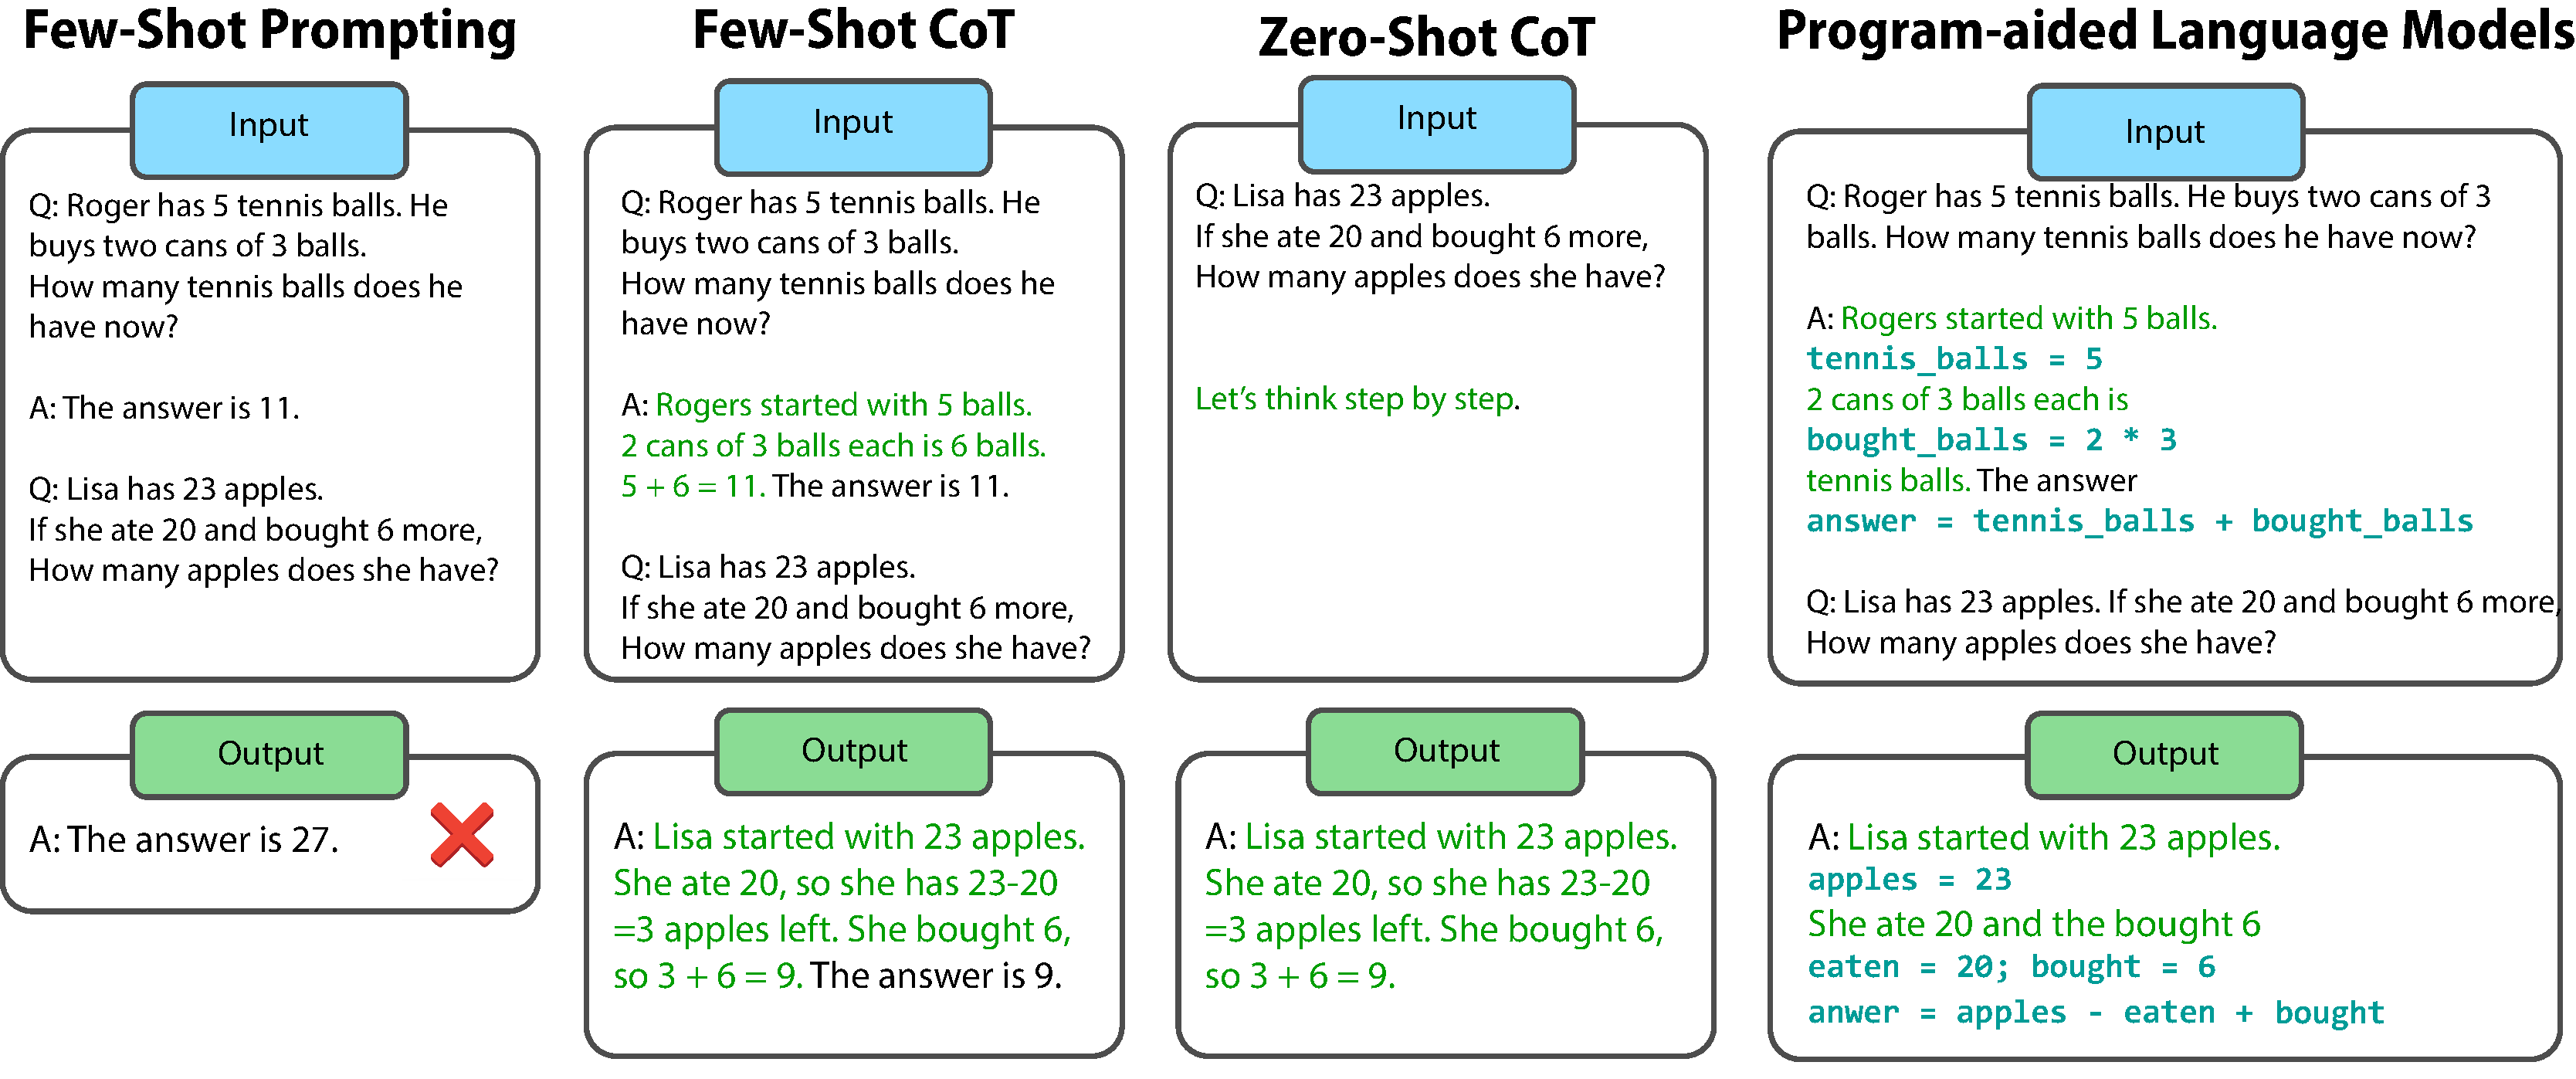
\includegraphics[width=\textwidth]{figures/cot2.pdf}
    \caption{不同的思维链（CoT）提示技术 \citep{wei2022chain,kojima2022large,gao2023pal,plaat2024reasoning}。上方是提示词，下方是答案。}\label{fig:cot} \label{fig:zero} \label{fig:pal} 
  \end{center}
\end{figure}


「只要给出提示，LLM 就能被引导去遵循分步指令」这一想法引起了极大的兴奋，也开启了关于 LLM 多步推理的进一步研究。此后，思维链（CoT）已成为 LLM 中一种标准的提示方法。

在
原始论文中，提示词由
研究者针对各类问题手工编写。
\citet{kojima2022large} 更进了一步。
他们表明，仅仅加上一句与任务无关的话（{\em 让我们一步步思考}），也能
显著提升许多问题的表现。由于这段文字不含与问题相关的要素，它属于一种零样本学习。
图~\ref{fig:zero} 比较了这些方法（第二列与第三列）。
实验还表明，加上这句话之后，在其他推理基准上也取得了显著的性能提升，
包括算术、符号与逻辑推理（在使用更新的 PaLM LLM、并同时加入自洽性（见下一节）时，在 GSM8K 上达到 70\% 准确率 \citep{wang2022self}）。

思维链这一想法本身受 Scratchpad \citep{nye2021show}、其他早期为算术推理生成自然语言
步骤的工作
\citep{ling2017program,cobbe2021training}，以及使用形式语言进行推理的工作~\citep{roy2016solving,chiang2018semantically,amini2019mathqa,chen2019neural} 启发。


\begin{comment}
    
\paragraph{Self Generation}
In contrast to manually writing prompts we can also let the
LLM itself write a multi-step reasoning-prompt.
An example of such self-improvement is auto-chain of thought
\citep{zhang2022automatic}.  
First, auto-chain generates specific questions for a
given dataset and partitions them into  clusters. Then an external algorithm uses the model to generate examples that are sampled for diversity. The constructed demonstrations augment the original prompt.
In an experiment with GPT-3, this approach improved hand-written chain of thought prompts by a few percentage points better, on ten benchmarks \citep{zhang2022automatic}.

\end{comment}

%\subsection{Self Evaluation}
%
%\citet{fu2022complexity} introduce Complexity-based
%prompting. Inspired by Chain-of-thought and Self-consistency, %this
%work studies which prompts achieve the best results on math word and
%other reasoning problems.
%their work specifically studies the impact of the complexity  of the
%reasoning chain (the number of steps), and introduces a related reasoning approach (Complexity-based prompting).
%They find that prompts with the largest
%complexity  perform best, and also that  answers with the highest complexity are the best.  Complexity-based prompting
%achieves somewhat higher performance on three math reasoning benchmarks: GSM8K improves 7 points, MathQA 6 points, and the Penguins benchmark from Big Bench Hard improve 3 percentage points. 

%We see that the initial approaches showed larger  improvements than the later approaches. It is time to look at another category of approaches, that focus on the evaluation of reasoning steps.

%Another approach that uses model-generated prompts is Buffer-of-thoughts. We will discuss this approach in Section~\ref{sec:buffer}.


\subsubsection{自我评估}
%\paragraph{Evaluation of Steps}
LLM 并不完美，结果中会出现错误。
当生成多个推理步骤时，错误会累积。为防止错误失控，我们应当格外注意对结果的评估。
%
下面我们考察一些减少错误累积的方法，它们要么通过检查模型本身，要么通过评估中间推理步骤。



当 LLM 被提示进行 CoT 推理时，它们会
执行一连串步骤。执行多个步骤使它们
对错误敏感、容易发生错误
累积 % (logical, factual, ethical, or otherwise)
\citep{weng2022large,xiao2023survey}。人们已发展出若干方法来防止错误
累积。一种做法是另建一个模型来单独
评估结果。%\citet{shen2021generate} and \citet{li2022advance} train an external verifier to check  results.
%
%In contrast, 
\citet{weng2022large} 提出了一种由同一个 LLM 进行评估的自动化方法，称为自我验证。%They note that human reasoning also suffers from the  problem of accumulating errors, and that in human reasoning we frequently revisit our thought process to verify the accuracy of our reasoning steps. % Thus, they propose to apply such a backwards self-verification approach. 
其做法是提示 LLM 把
思维链推理链的结论作为
求解原问题的条件，然后回到原问题
去比较答案。LLM 会得到自己结论的若干变体，并被要求选出与
原问题相似度最高的那一个。%(Note that there can be feedback issues using an LLM to evaluate itself, for a discussion see \citet{zheng2024judging}.)
% Experiments are reported on GPT-3 \citep{chen2021evaluating} and on Instruct-GPT \citep{ouyang2022training}. The accuracy of Chain-of-thought was improved by a few percentage points on arithmetic  and general reasoning tasks (GSM8K 65\%, AQuA 48\%, SVAMP 77\%). 




一个流行的相关方法是自洽性 \citep{wang2022self}。\label{selfconsistency}
自洽性是一种集成方法（一种著名的机器学习技术，通过组合多个较弱的
学习器来得到一个强学习器 \citep{sagi2018ensemble,breiman2001random}）。
传统上，LLM 查询的答案是通过贪心地沿着 logit 值最高的路径、从解码器网络中抽取出来的。在自洽性中，贪心的单路径解码被替换为在更广的路径样本上做多数投票。
通过对多样的推理路径进行采样、评估，并选出其中最具一致性的答案，自洽性实际上是在让 LLM 对同一个查询执行多次，再对 Transformer 模型的内部解码路径做多数投票。自洽性
之所以有效，是因为复杂的推理问题通常
存在多条通向
正确答案的推理路径。图~\ref{fig:sc} 给出了该方法的一个例子。
%
%
\begin{figure}
  \begin{center}
    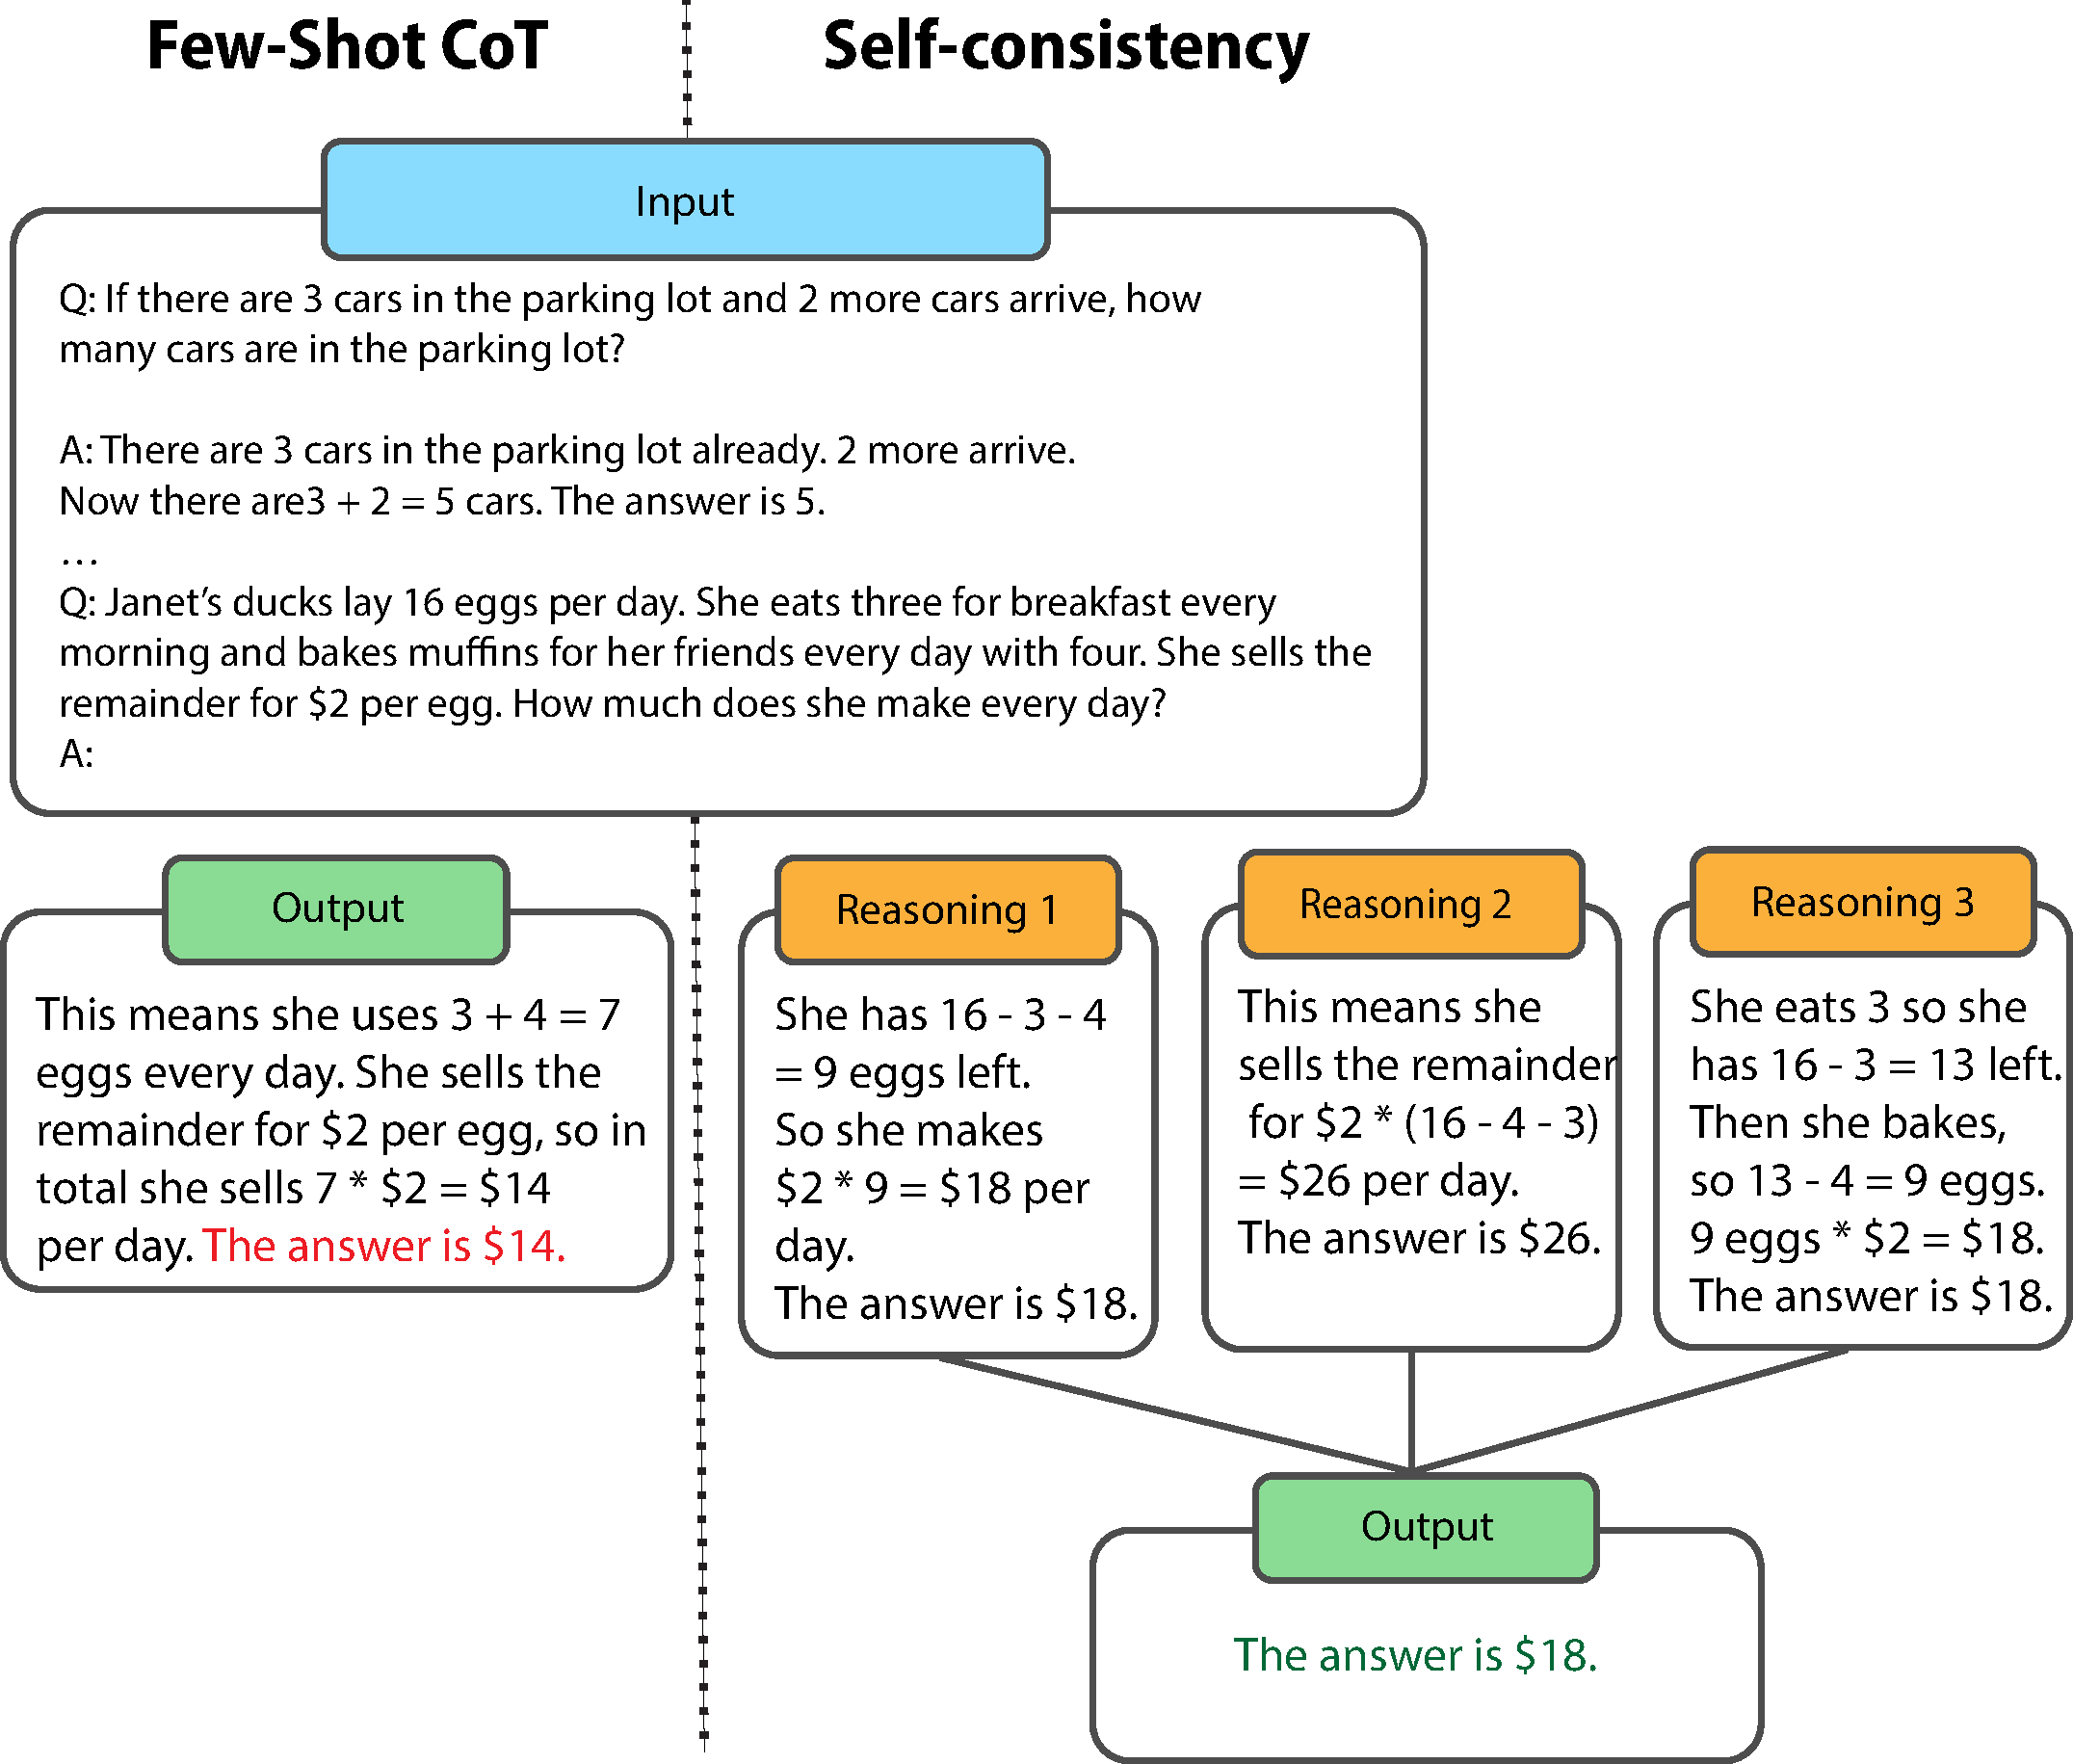
\includegraphics[width=10cm]{figures/selfconsistency.pdf}
    \caption{自洽性（改自 \citep{wang2022self}），展示多数投票}\label{fig:sc}
  \end{center}
\end{figure}
%
 
自洽性已在算术推理、常识
推理与符号推理上、配合多种 LLM（包括 GPT-3）做过评估。
%It is also compared against sample and rank, beam search, and ensemble approaches.
自洽性通常能在思维链的基础上
再提升 10-20 个百分点。在现代 LLM 中，自洽性常与思维链结合使用。% and approaches that we discuss in this book.
%(Self-verification also reports that
%performance is improved when used in combination with Self-consistency
%\citep{wang2022self} and with Program-aided-language \citep{gao2023pal}.)

\subsubsection{用代码生成来验证}\label{sec:selfdebug}

另一种提高推理步骤序列准确率的做法，是从自然语言转向形式语言。形式语言的优点
是比自然语言歧义更少。例子包括计算机语言（如 Python）或数理逻辑。


%\paragraph{Codex}
LLM 在从自然语言提示生成计算机代码方面相当成功。
\citet{chen2021evaluating} 提出了 Codex，这是一个在
GitHub 仓库中公开代码上训练的 GPT 模型。Codex 能够从
自然语言描述（如注释字符串）生成正确的程序。
%Figure~\ref{fig:codex} shows examples that are produced by Codex.
%
% \begin{figure}
%   \begin{center}
%     \includegraphics[width=12cm]{figures/codex}
%     \caption{Codex example \citep{chen2021evaluating}}\label{fig:codex}
%   \end{center}
% \end{figure}
%LLMs are well suited for generating computer code. 
此后，用形式语言进行推理成了一种流行做法。%The work on Codex is used as a basis for further research on reasoning in LLMs.
许多方法用 Python 生成推理步骤，这样代码就能被编译器、调试器或解释器求值。
人类程序员写代码时，通常
遵循这样的循环：写一些代码、编译并执行它来查找错误，
再用反馈改进代码。这种做法
例如被用于自我调试
\citep{chen2023teaching}。%Self-debugging teaches a large language model to  debug its generated  program code via few-shot demonstrations. 
它遵循同样的步骤：代码生成、
代码执行与代码解释。
%(see Figure~\ref{fig:debug}).
%
% \begin{figure}
%   \begin{center}
%     \includegraphics[width=10cm]{figures/debug}
%     \caption{Self-Debugging control flow \citep{chen2023teaching}}\label{fig:debug}
%   \end{center}
% \end{figure}
 %
自我调试能够% , without human feedback on
%the code's correctness or error messages, 
通过检查执行结果，发现它自己
代码中的错误，%that was generated by itself from 
还能用自然语言给出对所生成代码的解释。%It achieves strong performance: the text-to-SQL Spider benchmark improves 9 points,  and the C++ to Python Transcoder benchmark improves by 12 percentage points. 


%\paragraph{Program of Thought and Program Aided Language}
%Two other approaches that use a formal language are Program-of-thought  \citep{chen2022program} and
另一种方法是程序辅助语言 \citep{gao2023pal}，它用 LLM 生成 Python，再用解释器对结果求值。在这种做法中，问题被翻译成小块 Python 代码，随后可由解释器执行来解决问题。
%Program of Thought   and Program Aided Language  use the LLM to
%read the natural language problem,  and then generate Python programs as the
%intermediate reasoning steps.
%The approaches are similar although Program-aided-language uses generic prompts, and has been tested on more benchmarks. % and has been used in  other approaches.  
图~\ref{fig:pal}（第四列）展示了程序辅助语言方法。
%
% \begin{figure}
%   \begin{center}
%     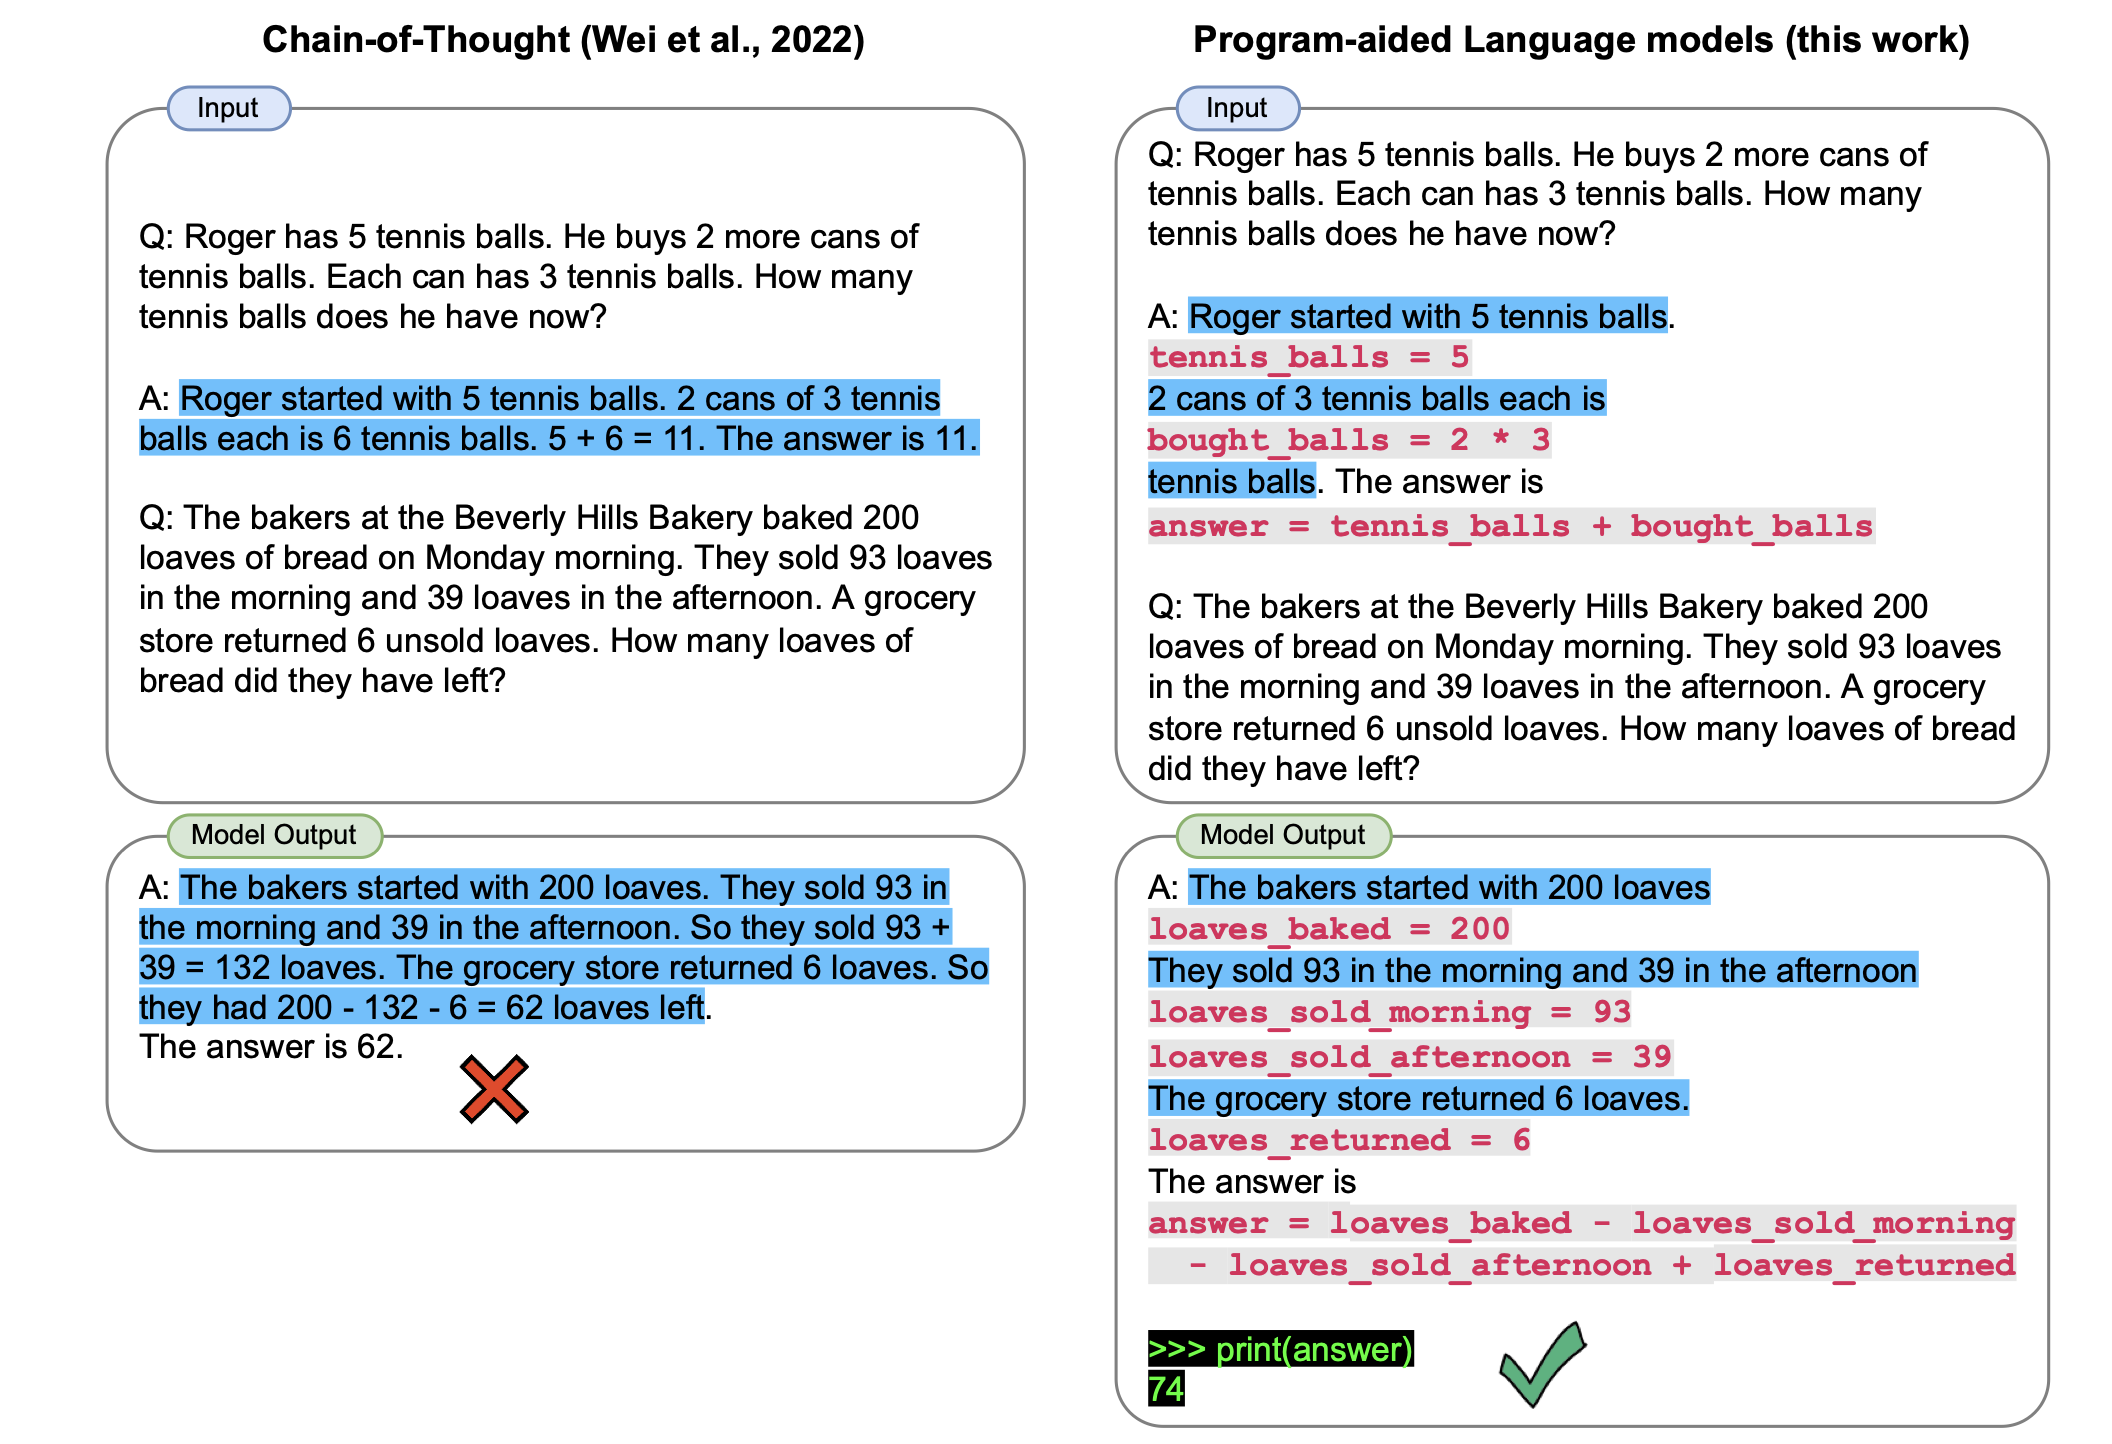
\includegraphics[width=11cm]{figures/pal}
%     \caption{Program-aided-language  \citep{gao2023pal}}\label{fig:pal}
%   \end{center}
% \end{figure}
%
当对推理步骤的求值被交给 Python
解释器之后，把自然语言问题分解为可执行的
代码步骤
就成了 LLM 唯一的任务。%(Earlier work in math word problems showed how to decompose a problem and reach an answer \citep{ling2017program}.) 
%
\citet{gao2023pal} 提供了大量实验
证据，展示神经 LLM 与符号解释器之间的协同作用。
实验在 13 项数学、符号与算法推理
任务上进行，取得了比当时大得多的
模型更准确的结果（例如，程序辅助语言在 GSM8K 上报告 72\%、在 Penguins 上报告 93\%）。%Mathematical word problems have been studied for some time.  




% FunSearch \cite{romera2024mathematical}
% \todo{FunSearch}

% LLaMEA \cite{van2024llamea}
% \todo{LLaMEa}

\subsubsection{演化式代码生成提示}
用形式语言做验证的工作，催生了若干自动生成可用代码、并针对特定问题调优而不需人工反馈的研究。
\citet{romera2024mathematical} 提出了 FunSearch，一种把形式方法与 LLM 结合起来以增强数学推理与代码生成的方法。FunSearch %is capable of producing functionally correct programs that adhere to specified requirements. It 
采用遗传式方法，维护多个候选解（程序）种群，并用一个取决于问题规格的函数来评估它们。%In addition to the %problem specification in the form of an 
%evaluation function, also an initial program is given to the LLM in the first prompt. 
在评估了由起始提示生成的程序之后，会以迭代方式构造新的提示词——把按评估得分排序后选出的采样程序组合起来，再要求 LLM 生成新程序。
另一项工作利用演化计算方法来生成并优化演化算法 \citep{van2024llamea}。该方法名为 LLaMEA（大语言模型演化算法），
利用 LLM 来设计与优化演化算法。它用 LLM 生成初始算法结构，再通过变异与选择加以精炼。%This  enhances the efficiency of algorithm design, particularly in fields requiring innovative and adaptive solutions, 
据报道，在黑盒优化基准（BBOB）\citep{hansen2010black} 上准确率提升了 11 个百分点。



\section{自我反思与状态}\label{sec:state}
上下文学习已成为一种强大的新型少样本学习方法。当我们的少样本示例给出了推理步骤时，我们就能进一步提升 LLM 的能力。

本节我们将考察上下文学习的一些局限，
%. We will analyze what it cannot do, 
并探讨拓展这些局限的途径。
%
我们先讨论状态与记忆问题。我们将考察状态如何在多次相互独立的 LLM 调用之间传递、长上下文窗口，以及 LLM 是否擅长解决那些需要它们操作状态的问题。%We will discuss the ensuing knowing-doing gap, and how improve prompts automatically  by wrapping a simple loop around  the LLM calls. 




\subsection{LLM 是无记忆的函数}
上下文少样本学习利用的是 LLM 在提示词条件下检索知识的能力。指令与示例被提供出来，Transformer 架构则在它庞大的 $(K,V)$ 参数模型中找出答案（下一个词元）。有了思维链提示，LLM 就以提示词中给定的少样本推理步骤为条件。%, possibly translating the reasoning steps to a formal language such as Python. 

上下文学习以函数式方式使用 LLM，即对 LLM 的全部输入都放在提示词里。模型 $f$ 为输入提示词 $p$ 找出答案 $a$：$$f(p)\rightarrow a.$$
原则上，LLM 不会在两次调用之间保留信息（模型参数保持不变，也不存在带历史的全局变量）。如果我们想细化请求、把上一次调用的状态信息带到下一次，那么所有这些状态都必须由用户在新的提示词 $p'$ 中给出。模型本身早已把上一个答案忘得一干二净。

对聊天机器人而言，在每个新问题里重复整段对话历史，是一种笨拙而不自然的交流方式。在人类对话中，我们的交谈对象会记得上一句说了什么，无需我们显式复述（尽管记者采访政客时，有时会用这种办法来让他们不跑题）。
商用聊天机器人部分地通过系统提示词来克服这个问题：它们不可见地把上一次 LLM 调用的输出提供给新一次 LLM 查询的提示词。然而原则仍然成立：LLM 擅长为提示词找出联想式的下一个词元答案，却完全不擅长记住答案、像我们在通用计算机编程语言中所理解的那样操作变量状态。由于不改变任何参数，LLM 不会在调用之间记住上下文中的状态。

\subsection{检索增强与长上下文窗口}
LLM 的记忆问题还更深一层。查询所需的全部信息都必须放在上下文窗口里。而上下文窗口的大小是有限的，这就从根本上限制了单次查询能传达给 LLM 的信息量。当我们想要摘要一大段文本（例如一本书）时，这一限制就成了问题。% for applications where timely or information from large databases is needed, or 
此外，在第~\ref{sec:icrl} 节中我们将讨论上下文{\em 强化}学习方法，它通过把完整的回合历史存入上下文窗口来工作。简言之，人们需要能把更多信息传给 LLM 的方法。

在推理时扩展信息量最早的方法之一，是{\em 面向生成式 AI 的检索增强}（RAG）。RAG 让 LLM 调用外部数据，例如企业数据库或维基百科 \citep{lewis2020retrieval}。RAG 的用途还包括减少事实性幻觉，以及获取时效性强的信息，如金融或物流数据。RAG 将在第~\ref{sec:rag} 章讨论。


为把更长的文本传给模型，人们开发出了上下文窗口更长的 LLM。在标准 Transformer 架构下，算力需求随上下文窗口大小呈平方级增长，因此人们正在开发线性架构 \citep{ren2024samba}。另一种方案是压缩上下文窗口中的信息，例如用语义压缩 \citep{fei2024extending}、把信息分块 \citep{wang2023augmenting,zhou2025mem1}，或采用递归方法 \citep{zhang2025recursive}。
为 LLM 设计新颖的记忆架构是一个活跃的研究领域 \citep{yan2025general}。

\begin{figure}
    \centering
    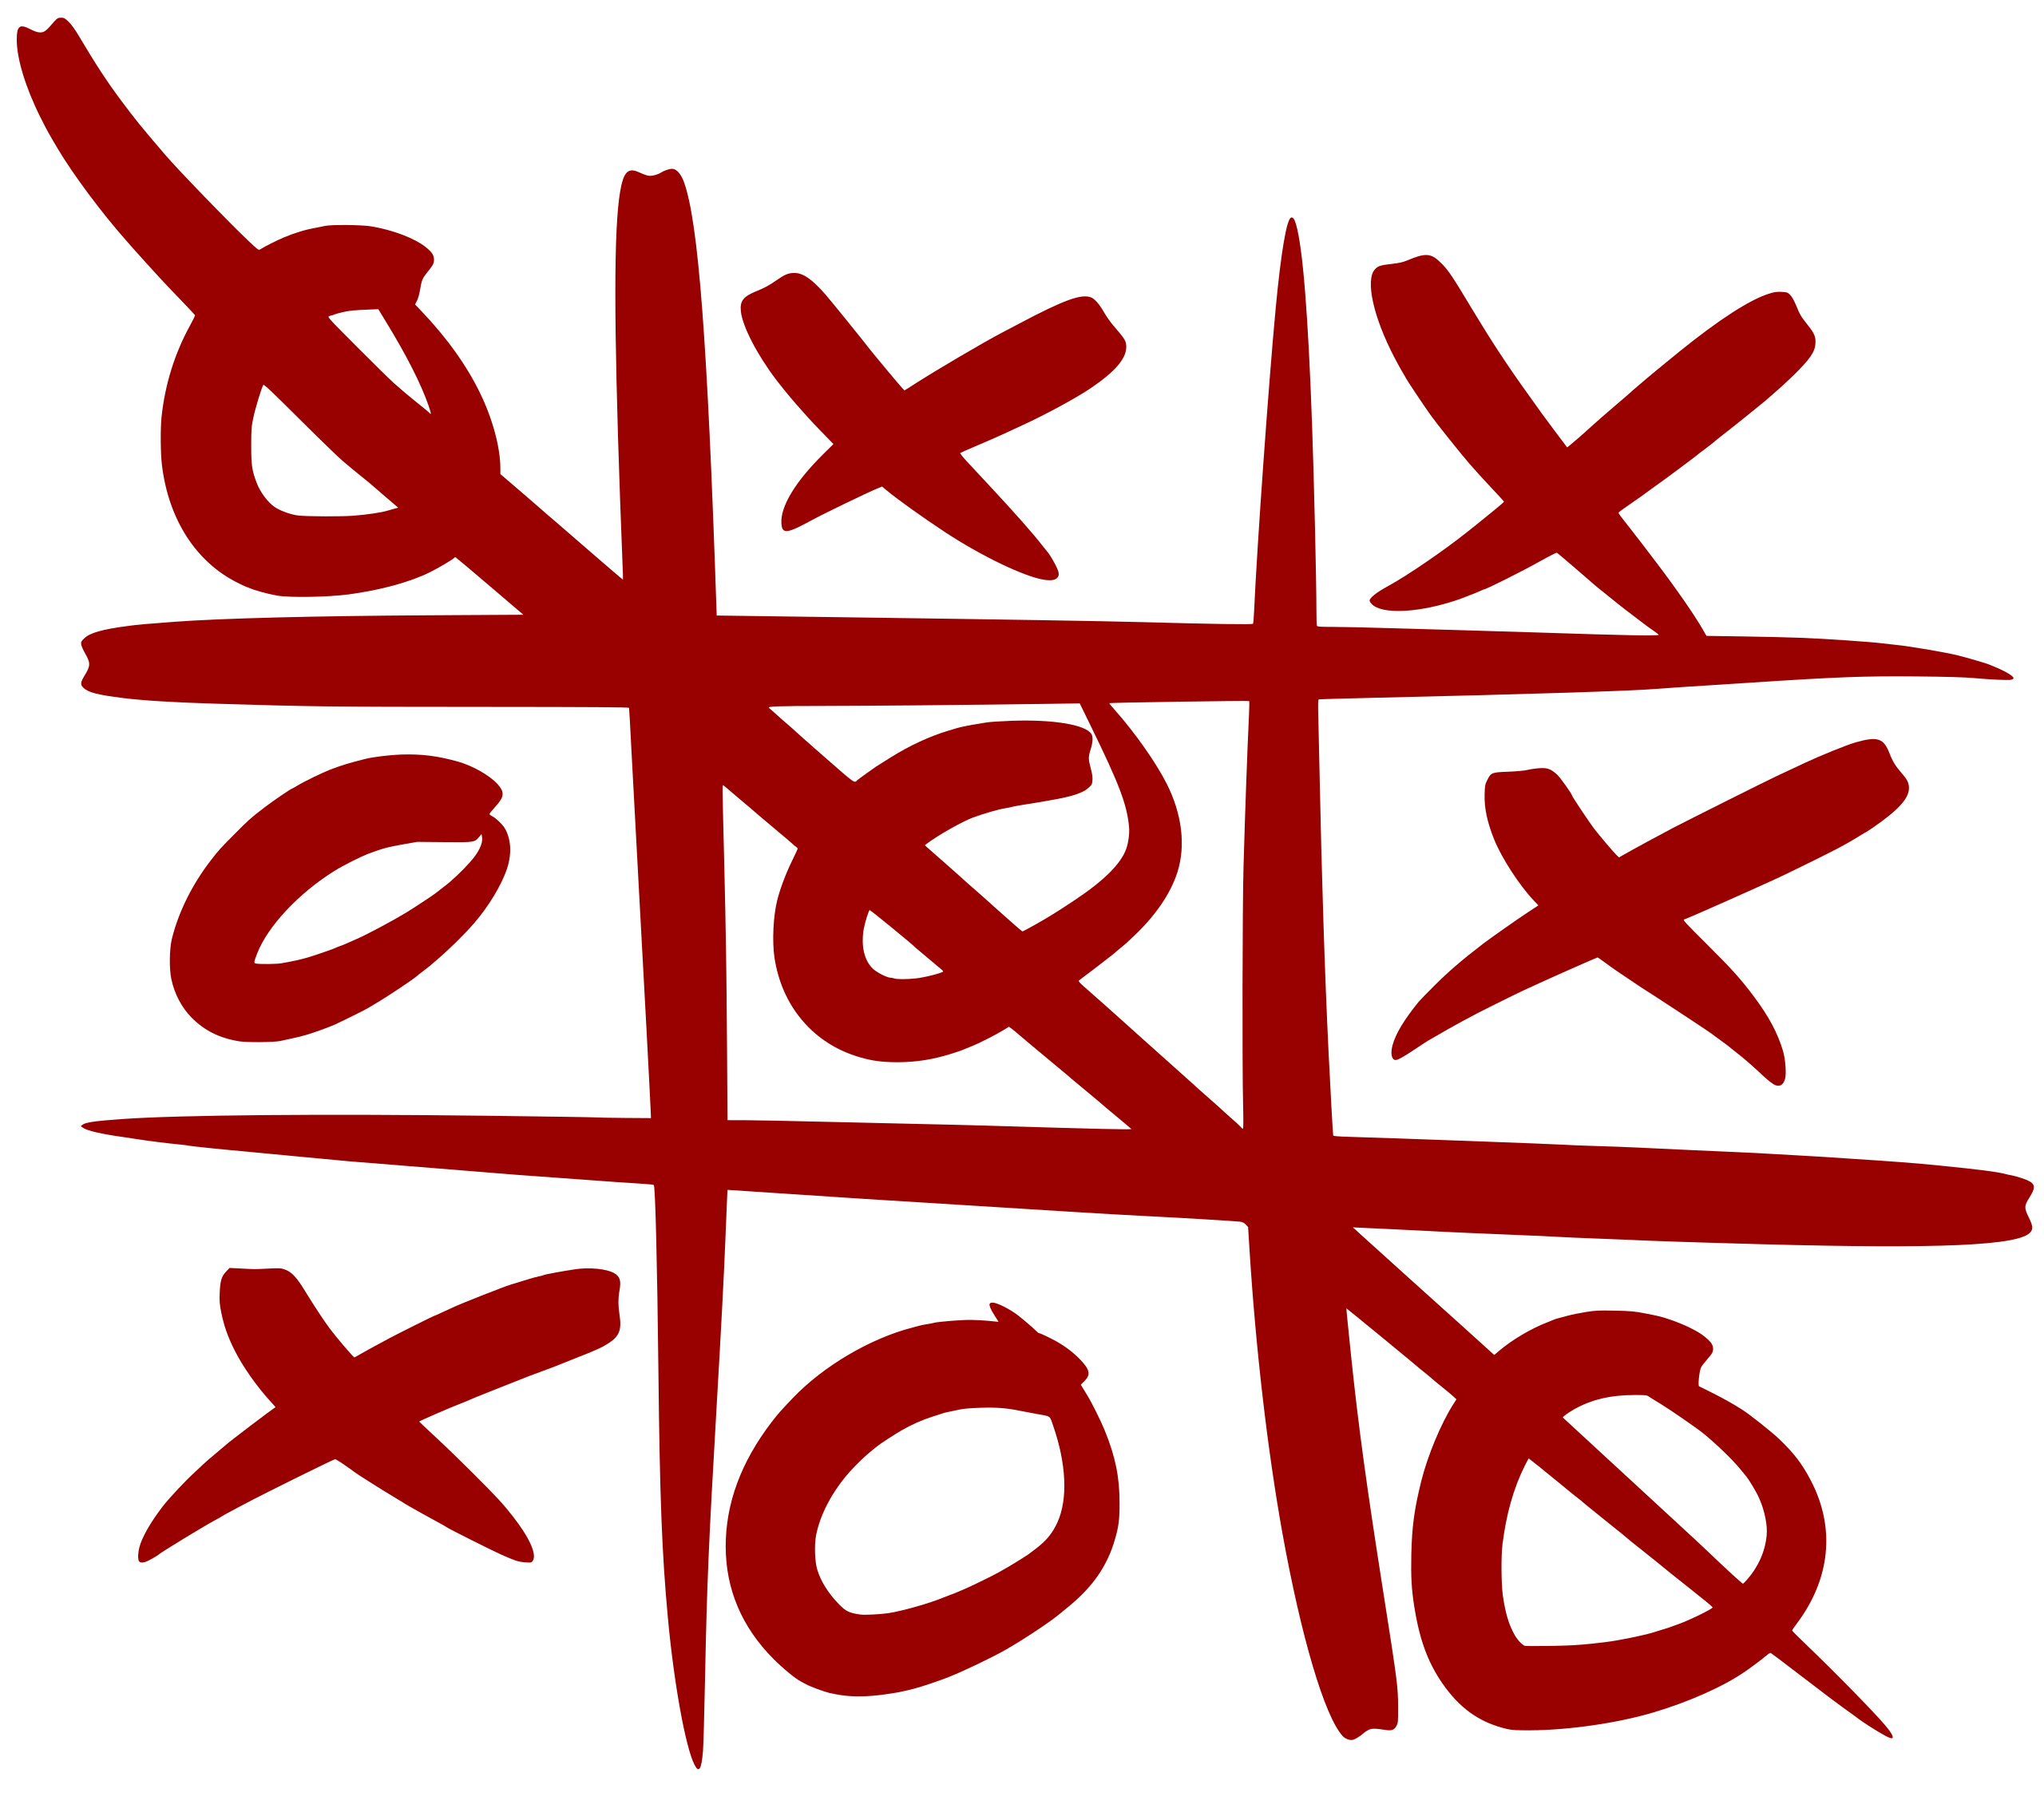
\includegraphics[width=0.35\linewidth]{figures/ttt}
    \caption{井字棋是一个简单的棋盘游戏，其中状态很重要}
    \label{fig:ttt}
\end{figure}

\subsection{LLM 与有状态问题}
LLM 在解决必须管理状态的问题上表现很差 \citep{wong2025towards}。例如在规划问题中，当前状态必须被准确记住——哪怕是图~\ref{fig:ttt} 所示那种简单棋盘游戏。LLM 容易把状态搞混，给出听起来合理、对训练语料中见过的局面可能正确、但对眼前实际棋盘状态却是错误的答案 \citep{paglieri2024balrog,ruoss2024lmact}。

人们尝试了许多方法来改进带状态的推理，其灵感往往来自强化学习与规划算法 \citep{wongstate}。
为了看清 LLM 如何被用来解决这类有状态问题，我们讨论一下 LLM 的无记忆特性如何使它们陷入一个称为{\em 知行差距}的问题。%We also briefly discuss if there are theoretical limits to what transformers can do. 
此外还发展出一些更高级的方法，让 LLM 能更好地处理有状态问题。第~\ref{chap:arch} 章将讨论这些高级途径。
%First we discuss the idea to pretrain models on decision traces. Next, we discuss methods that optimize prompts externally using search methods, and using learning-based methods, using an agentic harness (self-reflection). %We discuss in-context  reinforcement learning (ICRL), and self-reflection.
%Finally, we discuss implicit reasoning methods. 

\paragraph{知行差距}\label{sec:knowing}
除了 LLM 调用{\em 之间}缺乏状态之外，还有一个与记忆有关的问题，出现在 LLM 对某些任务的{\em 内部}执行过程中。

这个问题被称为{\em 知行差距}。它描述的是一种奇特现象：LLM 能够生成一段正确的文字描述来解决问题，甚至给出正确的算法，却无法正确地执行这个算法 \citep{paglieri2024balrog}。当你问 LLM 如何解决某个问题时，它能立刻给出可执行的 Python 代码形式的正确算法。可当你随后要求它真正解决这个问题时，LLM 却不能正确遵循它刚才生成的算法。错误往往出现在它所生成算法中变量发生状态变化的地方 \citep{paglieri2024balrog,ruoss2024lmact}。要注意，逐步忠实地执行算法代码、追踪寄存器中的取值，根本不是 LLM 中基于注意力的 Transformer 所设计的目标——它们的设计目标是通过某种联想记忆来模拟自然语言处理 \citep{la2024code}。\footnote{还要注意，人脑有时也有同样的问题：我们很容易描述长除法的算法，但被要求计算 $12345/42$ 时可能会出错——计算机擅长这个，人类不擅长，LLM 也不擅长。}

除了知行差距，还有另一个状态管理问题。
%The $(K,V)$-transformer architecture is good at functional (input-based) associative retrieval, but not at meticulous state manipulation. 
提示 LLM 与自己下棋走前几步，可能会看到棋盘上的棋子神奇地消失或出现。模型意识不到自己走的那些棋步在某些局面下也许不错，却不符合当前棋盘位置，甚至还会用聊天式的语气给这些错步配上一个听起来合理的理由。%Playing a sequence of moves in a board game, an LLM strings together good moves that it has seen before in similar situations, without critically checking  if the board positions match exactly.  
LLM 难以可靠地管理一个变量从一个值转移到另一个值的状态变化。单个取值容易被遗忘或搞混。可以在提示词中插入额外文字，指示模型在走下一步之前仔细追踪变量取值 \citep{la2024code}，但这是笨拙且易错的办法。%Such extra texts take up valuable space in the context window, and slow down inference. To ensure correct gameplay,  additional text can be inserted into the prompt to instruct it to carefully carry over the correct board state when making a next move.

知行差距与棋子消失问题，都可以通过调用外部解释器来执行 LLM 生成的算法而绕开。商用聊天机器人有时会采用这一策略。这是个聪明而实用的方案：除了能正确执行 Python 代码之外，Python 解释器还会比 LLM 更高效。

第~\ref{chap:arch} 章将讨论在 Transformer 架构中处理状态与记忆的其他途径。

\subsection{用于改进提示词的智能体运行框架}\label{sec:self-reflection}\label{sec:inferencetime}
%Although decision-trained transformers can solve small planning tasks, losing the ability to converse in natural language with our models is often problematic, and, in LLMs,  the knowing-doing gap for planning problems remains an open problem. 

除了求助于外部执行生成的代码之外，人们还发展出其他方法来处理记忆与状态。在本节中，我们将%discuss agentic solutions for state management.
%We will now return to LLMs, to models that are trained on language. 
%We will 
转向智能体式做法，引入小型外部算法来显式地管理状态与提示词。这样的算法称为{\em 运行框架}。运行框架还可以让同一个 LLM 扮演不同角色、为每个角色配以不同的提示词，例如用于状态的{\em 生成}或{\em 评估}。我们先从基于搜索算法的提示词管理谈起。
%In the next subsections we will see whether LLMs (transformers that are pretrained on natural language) can also do reinforcement learning at test time---in addition to transformers that are trained on decision traces---since it would be convenient to be able to communicate with our agents in natural language. 

当 LLM 以不同角色被调用时，例如去批判（评估）它自己刚刚生成的表现，就可以说 LLM 在进行{\em 自我反思}。这个略显拟人化的说法在文献中被广泛用于这类方法。究竟是谁（而非什么人）在做自我反思——是 LLM 还是智能体运行框架——仍有争论。


\subsubsection{基于搜索的提示词优化}\label{sec:planning}
%\subsubsection{Self Reflection}
下面我们讨论基于搜索的推理时决策方法。
这些是超越思维链的上下文学习方法。思维链探索的是单条推理步骤链，每一步只有一个后继步骤。基于搜索的方法则在每一步探索多个选项，从而形成一棵可能性之树。

当我们想考察一棵可能的推理步骤之树时，就需要一种方法来跟踪：我们看过哪一步、目前最好的答案是什么、还有哪些步骤需要进一步考察。如前所见，LLM 并不太擅长跟踪状态，而常规计算机算法（比如一小段 Python 代码）却很擅长。
%In reasoning, often multiple valid  steps are possible, but pursuing all possibilities over multiple trajectories may lead to an infeasible number of possibilities. %We can use optimization algorithms to search through the space of possibilities in a smart way. 
%We can use an external prompt management   controller algorithm to do so. 
%For example, 
%Suitable options are standard tree search algorithms or  a reinforcement learning loop algorithm, can be used % to guide the search through the space of possible steps \citep{sutton2018reinforcement,kaelbling1996reinforcement,plaat2020learning}, as a harness. 
%
%\todo{\bf PROVIDE CODE FOR TREE SEARCH AND FOR RL?}
%
%This group of control approaches enables the most elaborate control of the reasoning process, and is used by many works, as we will see. 
这样的算法会把问题分解为一棵搜索树，其中会生成多个备选步骤，可以向未来搜索多步（见图~\ref{fig:tot}，位于第~\pageref{fig:tot} 页）。这些算法把 LLM 当作子程序调用，提示它执行诸如动作选择与奖励评估之类的任务。随后算法可以回溯，尝试其他备选步骤。这个控制算法位于 LLM 之外。它包裹在 LLM 外面，负责跟踪状态、管理提示词，并把 LLM 与外部世界隔开（也把外部世界与会搞乱状态的 LLM 隔开）。这个控制算法就称为{\em 运行框架}。
%
%Where greedy and ensemble processes can be controlled with a prompt by the LLM, this third category is more complex, and an external algorithm is used to control the reasoning process. 
 %The external algorithm allows more complex reasoning control, but we are now beyond prompt-based self-reasoning: control has been given to an  algorithm that is external to the LLM and external to prompt-learning.

我们从深度优先与广度优先搜索开始讨论控制策略 \citep{cormen2022introduction}。%then go to beam search, 
%and then to full reinforcement learning.
%
%\paragraph{Breadth first search}
\label{sec:buffer}
%A complex reasoning space can be traversed with a search algorithm.
%Where Chain-of-thought  creates a single prompt with a static sequence of reasoning steps over sub-problems, another approach, 
思维树 \citep{yao2024tree} 使用广度优先或深度优先搜索来动态地沿不同推理步骤前进。\footnote{思维树是一种流行的方法。Huggingface 链接在此：\url{https://huggingface.co/blog/sadhaklal/tree-of-thoughts}} %When one reasoning path has been traversed, the algorithm can backtrack, and try an alternative path. %The search control is executed with an external algorithm, t
%The paper describes both a breadth-first-search and a depth-first-search controller.
%
思维树中，生成（红色）与评估（绿色）两部分都由提示 LLM 来完成，见图~\ref{fig:totcode}。
%
\begin{figure}
  \begin{center}
    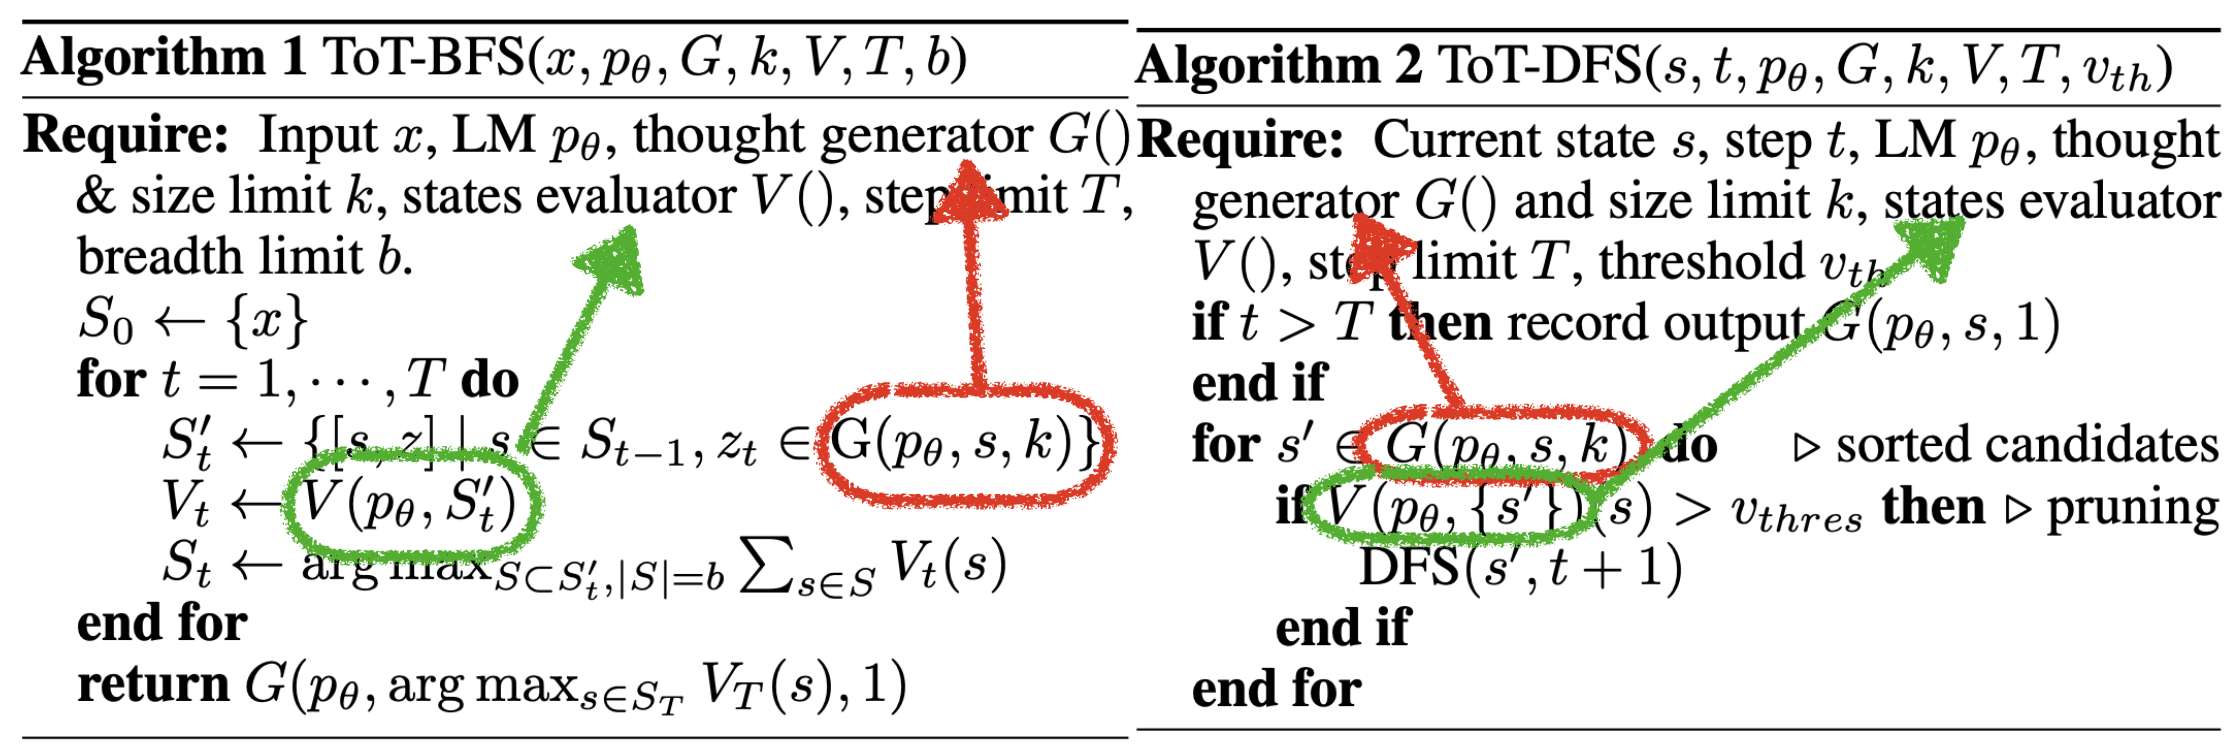
\includegraphics[width=12cm]{figures/totcode}
    \caption{思维树。左为广度优先搜索，右为深度优先搜索。箭头表示 LLM 提示（据 \citep{yao2024tree}）} \label{fig:totcode}  
  \end{center}
\end{figure}
%
两个 LLM 提示与外部控制结合起来，
使得对推理步骤空间的系统性探索成为可能，可以前瞻与回溯。%\todo{Should give example prompts for Generation and for Evaluation for a suitable example game}

\begin{figure}
  \begin{center}
    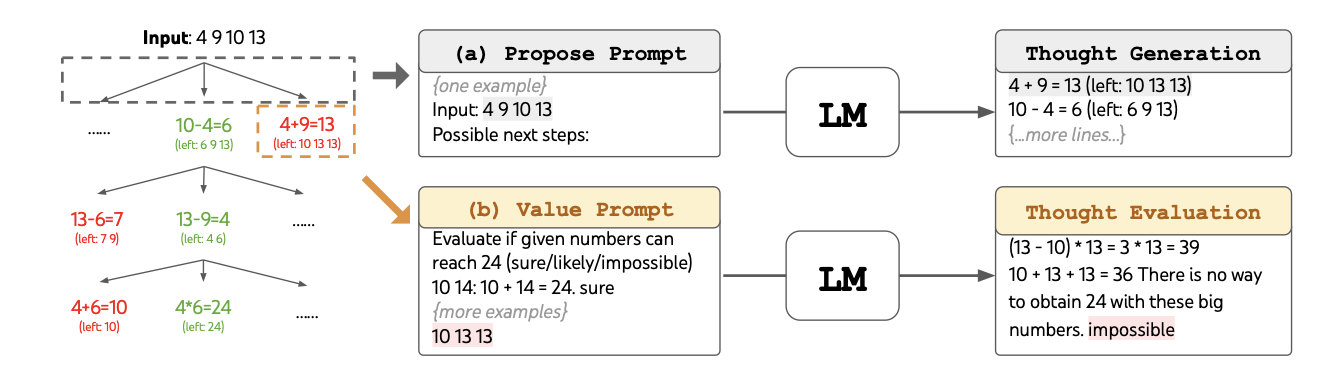
\includegraphics[width=12cm]{figures/tot-ex}
    \caption{思维树用于 24 点游戏的示例提示 \citep{yao2024tree}} \label{fig:tot-ex}  
  \end{center}
\end{figure}

思维树（ToT）已被用于 24 点游戏这类基于规划的谜题。在这个游戏中，给定 4 个数字，任务是在数字之间使用算术运算符 $( + - * / )$ 得到 24。例如，对数字 $4$ $9$ $10$ $13$，一个解是 $(10-4)*(13-9)=24$。思维树先用{\em 提议}提示生成一个局面：\verb|Input 4 9 10 13; Possible next steps:|，模型据此生成可能的下一步想法。随后这些想法由模型用带有思维链示例的评估提示来评估。图~\ref{fig:tot-ex} 展示了原论文中一个可能的提示序列。

作者把他们的方法与传统的线性思维链加自洽性在 24 点游戏、创意写作与迷你填字上做了比较，在 24 点游戏任务上取得 74\% 的准确率。其他任务则做定性评估。%Chain-of-thought builds a reasoning out of a path of thoughts,
% Self-consistency creates an ensemble of thoughts, and Tree-of-thoughts constructs a tree structure. 
图~\ref{fig:tot} 展示了这些不同的推理结构。\footnote{名字相近的另一种方法是思维图 \citep{besta2024graph}。思维图允许更一般的推理图，提供了一个形式化框架，其中各元素可以人工指定。}

\begin{figure}
  \begin{center}
    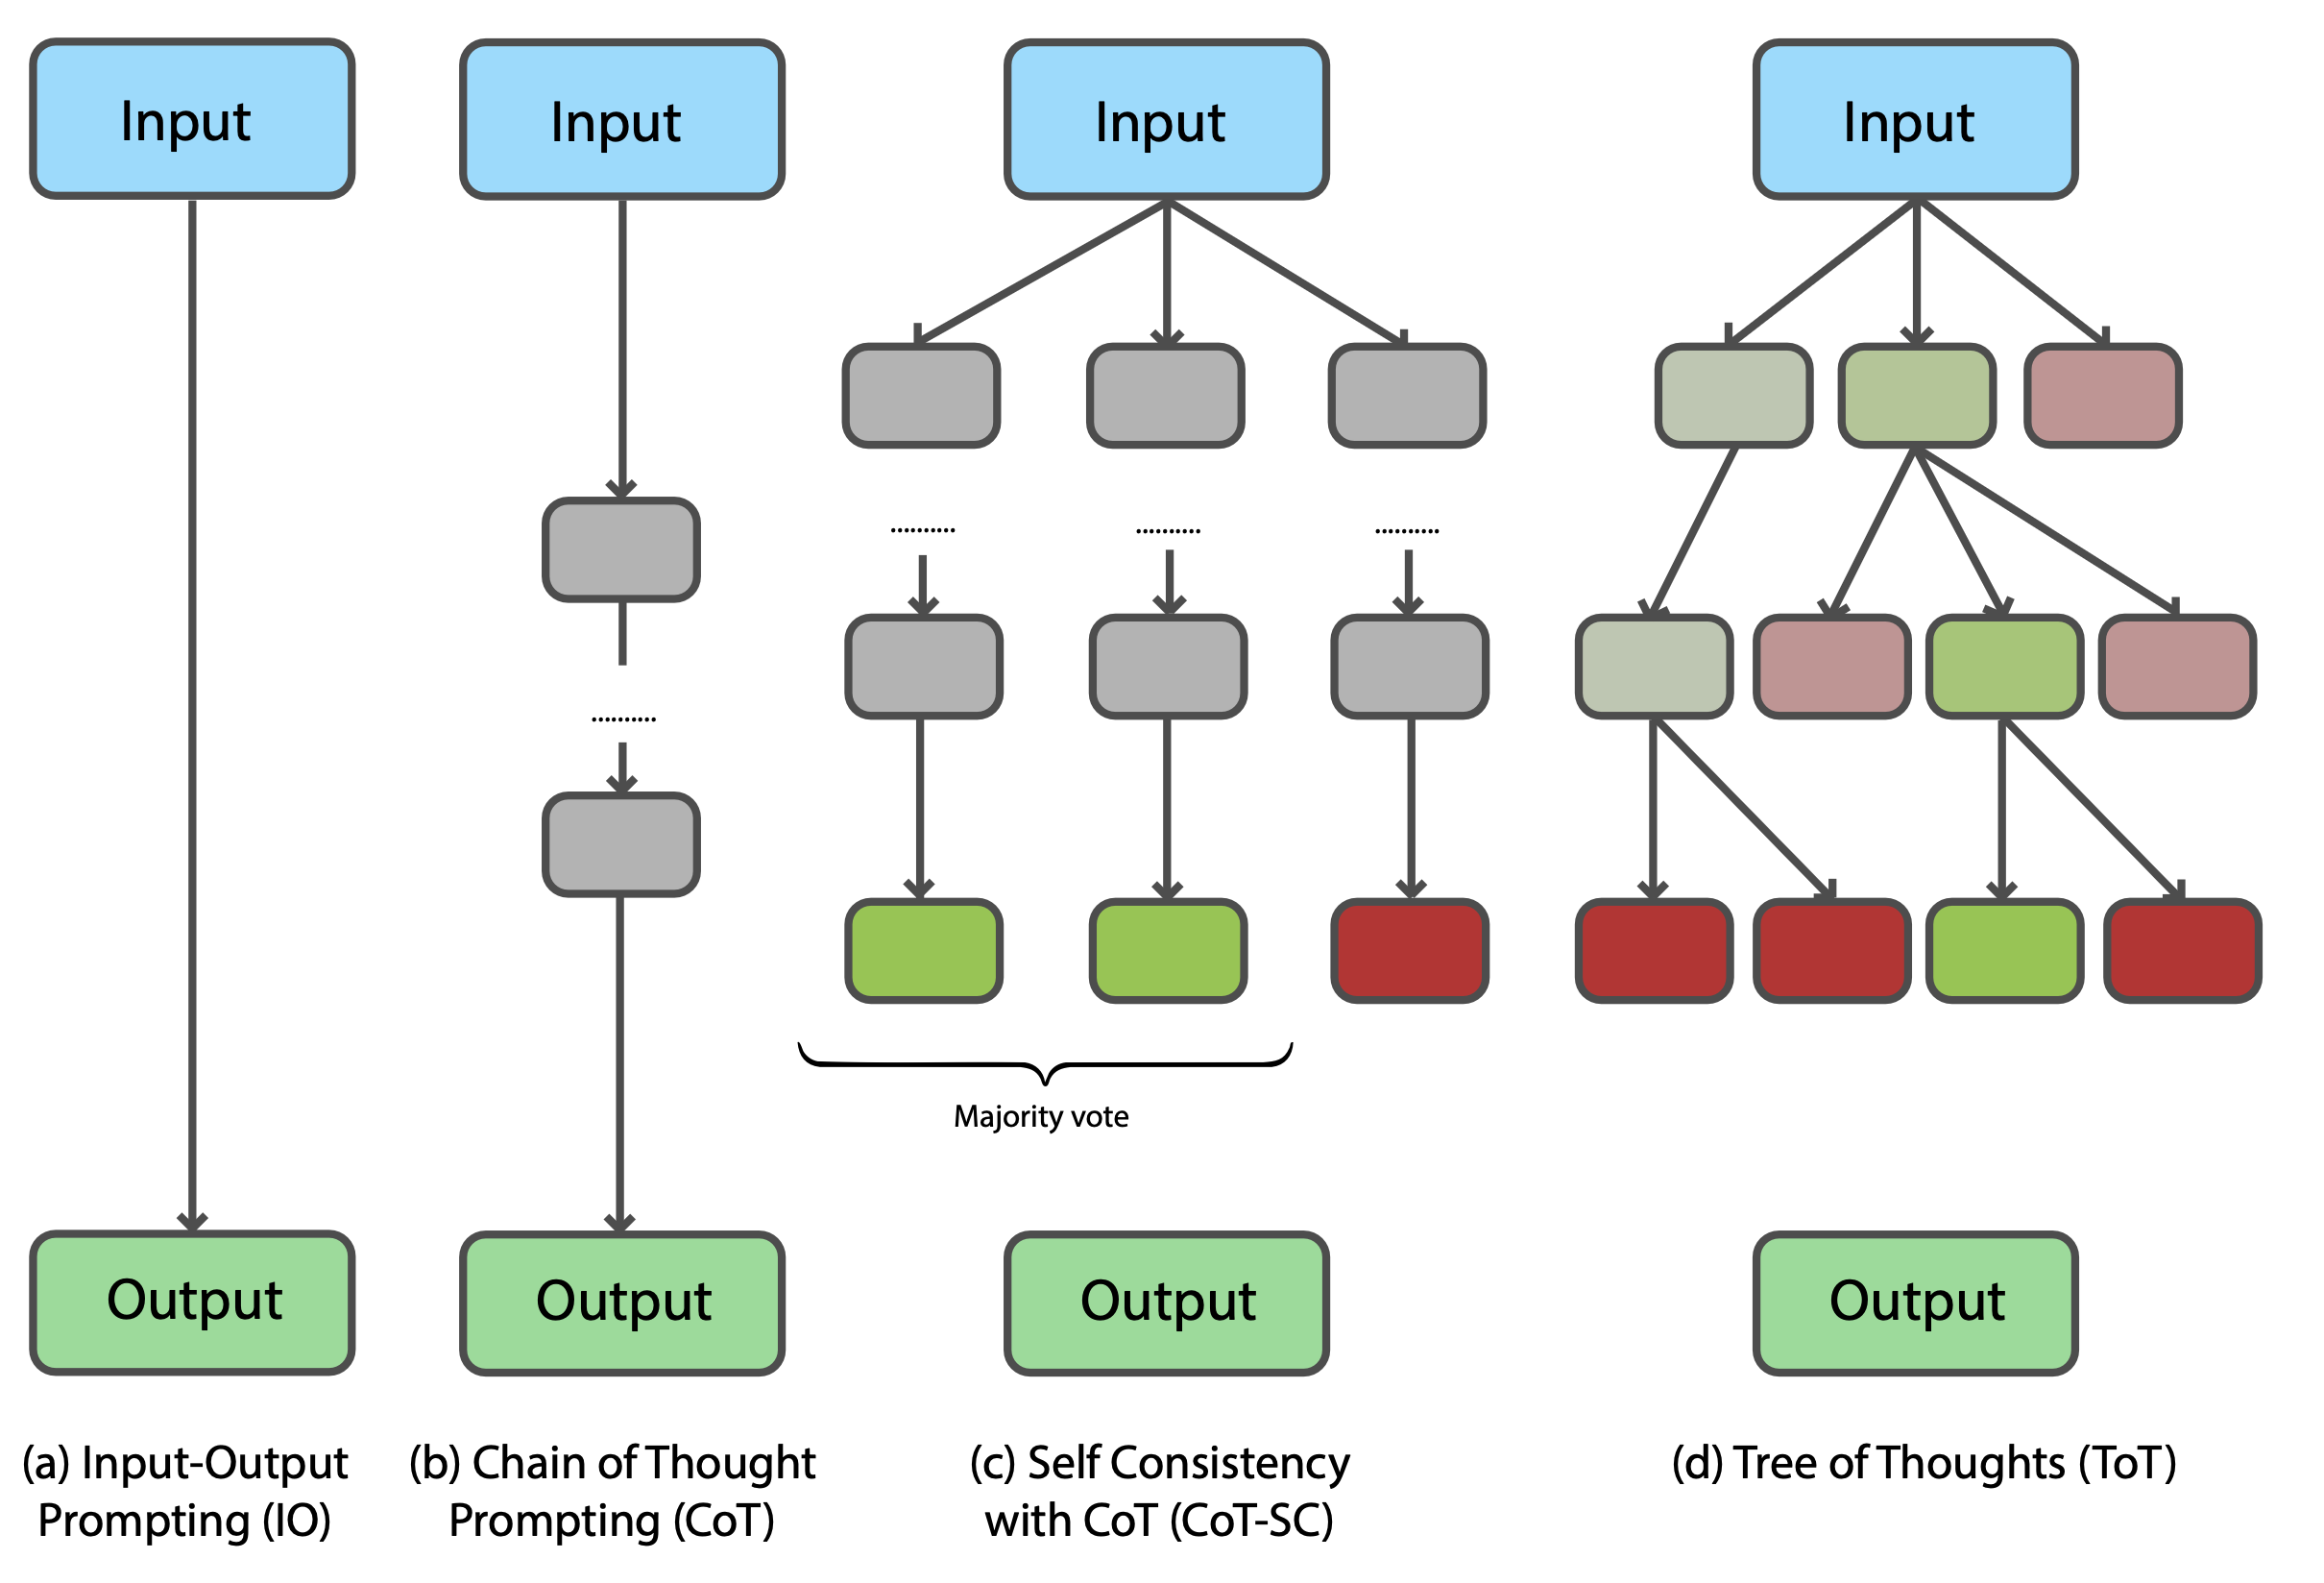
\includegraphics[width=\textwidth]{figures/cot-tot}
    \caption{思维链（b）、自洽性（c）、思维树（d）的推理结构} \label{fig:tot} \label{fig:bot}  
  \end{center}
\end{figure}

思维树是一种优雅的方法，在 LLM 之上叠加了两种最简单的搜索结构。提示序列易于跟踪，发现并纠正错误也很容易。

思维树的这两种搜索方法遵循固定的扩展策略。
接下来，我们将讨论更高级的、基于学习的方法，它们可能表现更好，代价是算法复杂度更高。

\subsubsection{自我反思}\label{sec:reflective}\label{sec:selfreflection}
人们设计了许多让 LLM 承担多个角色的方法。这类方法一般称为自我反思式方法。LLM 不仅被用来评估提示词，也被用来生成新的推理步骤，且常常对它们加以精炼。

自我反思这一领域还很年轻，新方法层出不穷。我们将介绍四种：自我精炼、ReAct、Reflexion 与思维缓冲。这些方法以不同方式使用 LLM，并借鉴强化学习的思路让 LLM 自我改进。

\paragraph{自我精炼} 第一种%other 
方法是自我精炼 \citep{madaan2023self}。该方法旨在借助反馈改进答案。%In this method, initial outputs from LLMs are improved through iterative feedback and refinement. 
%Like PHP, t
LLM 先生成一个初始输出，再为自己的
答案提供反馈，用 LLM 迭代地精炼自身。也就是说，LLM 被用来改进自己的答案，见
图~\ref{fig:refine}。
 %and \ref{fig:refine2} 
% illustrates the approach.
% %
% %
 \begin{figure}
   \begin{center}
     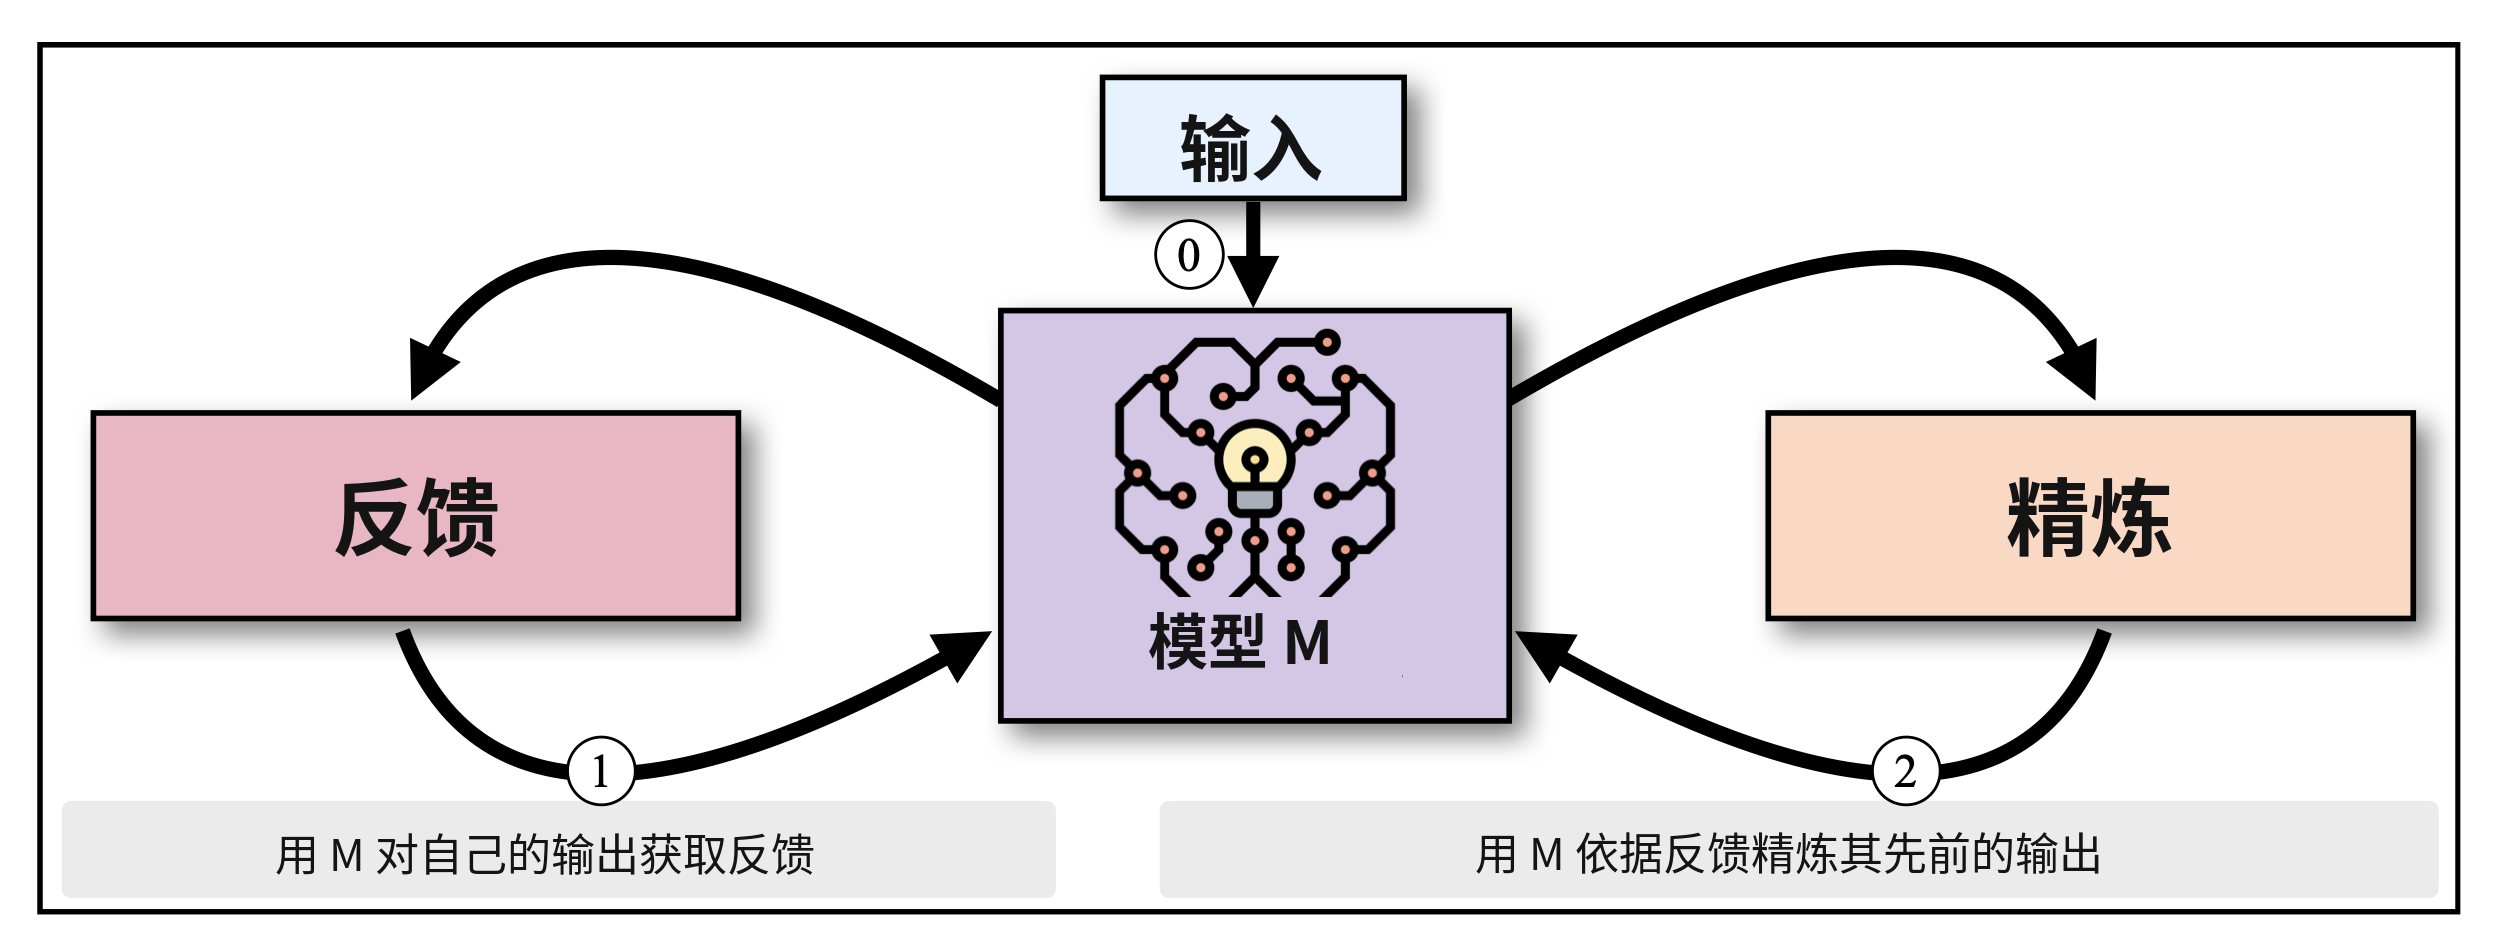
\includegraphics[width=9cm]{figures/selfref}
     \caption{自我精炼架构 \citep{madaan2023self}}\label{fig:refine}
  \end{center}
\end{figure}
% %
% \begin{figure}
%   \begin{center}
%     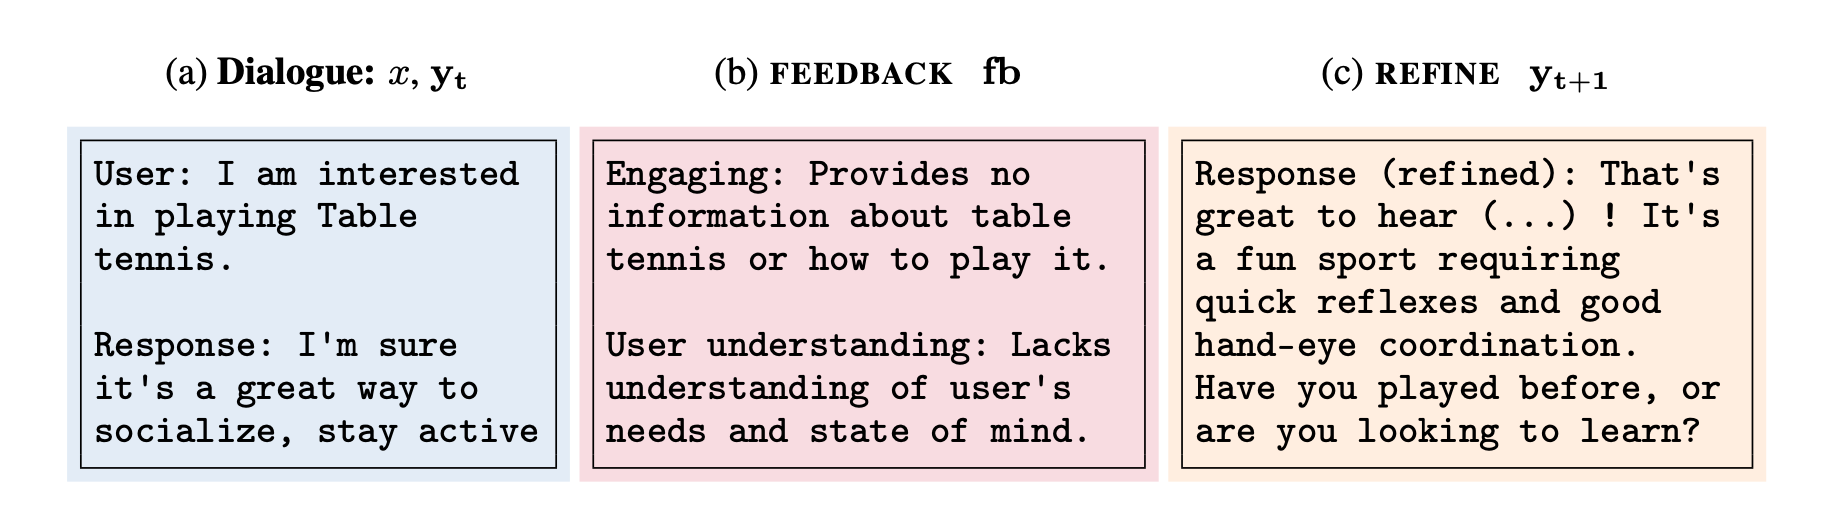
\includegraphics[width=10cm]{figures/selfrefine2}
%     \caption{Self-Refine Example \citep{madaan2023self}}\label{fig:refine2}
%   \end{center}
% \end{figure}
%
%The control flow of Self-refine is again governed by an algorithm external to the LLM and to the prompt. 
自我精炼以三种方式提示 LLM：（1）初始生成，（2）反馈，（3）精炼，遵循一条贪心的推理链。据报道，在对话
回复生成、代码优化与
受约束生成等基准上，自我精炼相比常规思维链有显著提升。这种做法确实遵循线性、贪心的推理链：在每个状态只尝试单个后继（不像 ToT 那样探索一棵树）。



\paragraph{ReAct}
把贪心做法加以推广，我们就可以用 LLM 在每个状态考察多个选项。
一个把强化学习与 LLM 结合起来的著名方法是 ReAct \citep{yao2022react}。\footnote{\url{https://github.com/ysymyth/ReAct}}
ReAct 把思维链提示学习作为强化学习框架的一部分，该框架还使用外部知识源（维基百科）与微调，用于减少错误、落地事实以及减少幻觉。该框架允许手工编写提示词。
%, but prompt allows human-written prompts and environment observations.
%
%On question answering (HotpotQA) and fact
%verification (Fever).
%ReAct overcomes 
%hallucination and error propagation in Chain-of-thought reasoning by
%interacting with a  Wikipedia API.
%, and, on the other hand, generating human-like
%task-solving trajectories that are more interpretable than baselines
%without reasoning traces. Furthermore,
% Figure~\ref{fig:react} shows four different
% prompting strategies.
% \begin{figure}
%   \begin{center}
%     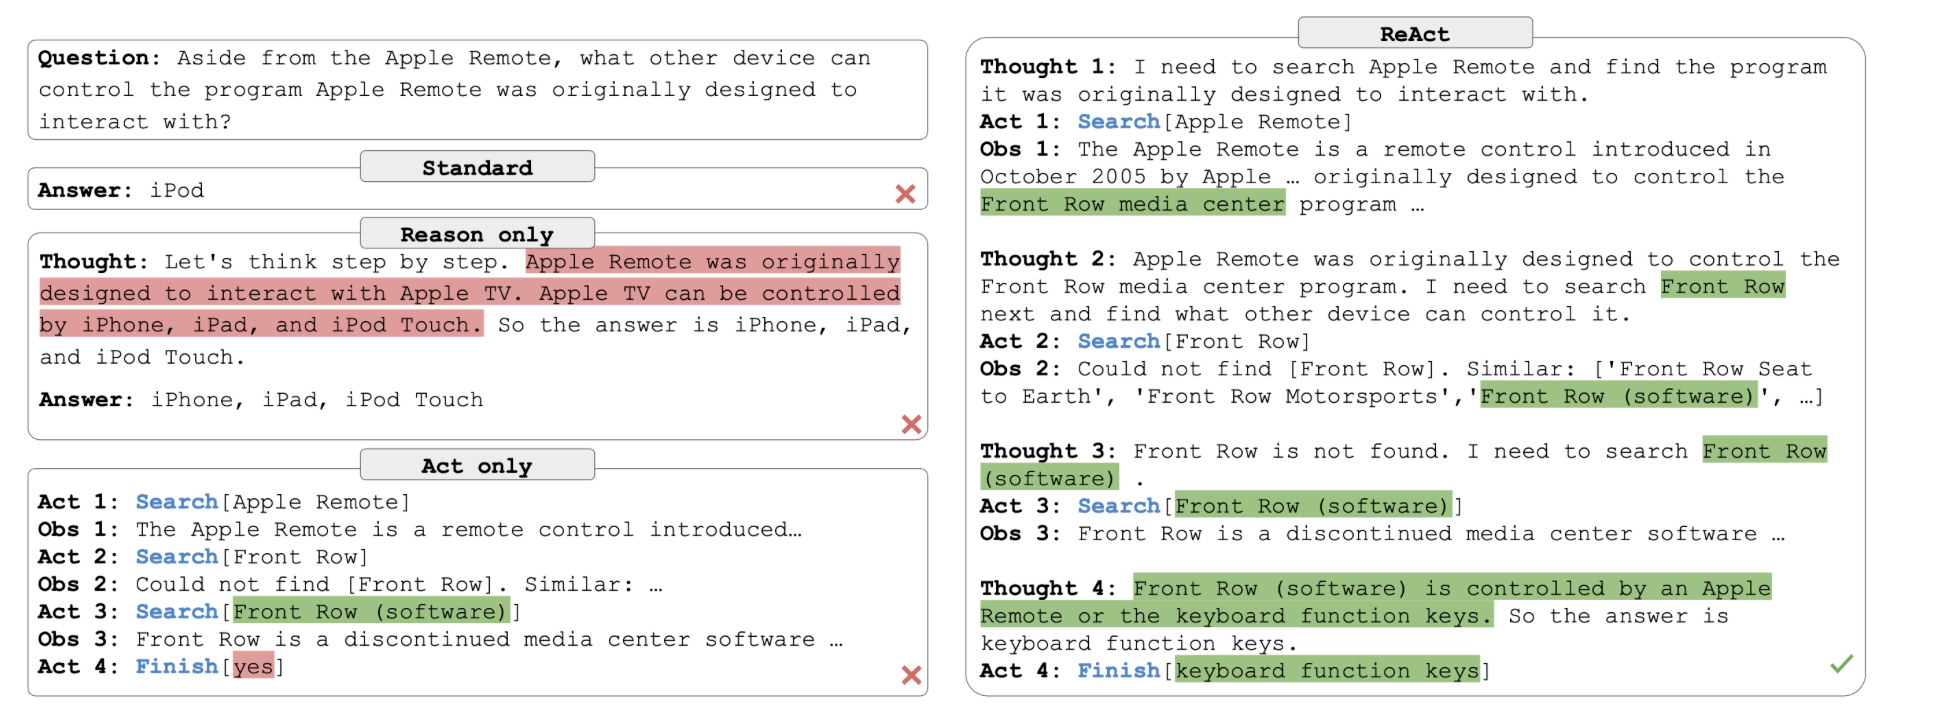
\includegraphics[width=12cm]{figures/react}
%     \caption{Comparison of four prompting strategies: Standard, Chain
%       of Thought (reason), Action only, and ReAct  \citep{yao2022react}}\label{fig:react}
%   \end{center}
% \end{figure}
%
%ReAct also experiments with finetuning of smaller language models
%using a teacher/student knowledge distillation setup.
在两个交互式决策
基准（Alfworld 与 WebShop）上，
ReAct 分别以 34\%
与 10\% 的绝对成功率超越了模仿学习
与强化学习方法。
%, while being prompted with
%in-context examples. 

\paragraph{Reflexion}
ReAct 的工作得到了进一步发展。
Reflexion \citep{shinn2024reflexion} %is a system for decision making (reinforcement learning) that 
%is a reinforcement learning system that 
%is built on top of ReAct. %Instead of a neural network with gradients, it is built on an LLM.
%Prompted by Reflexion, the LLM generates actions, to be executed in an environment.
%The goal is to 
创建能够通过反思失败来学习并
提升结果的 AI 智能体，其灵感来自人类做这件事的方式。\footnote{\url{https://github.com/noahshinn/reflexion}} 
Reflexion %is implemented as an external algorithm, that 
对 LLM 使用三个提示词：行动者、评估者与反思者。
% A notable extension is that 
Reflexion 运行框架在多次 LLM 调用之间加入了显式记忆。它有用于轨迹生成的短期记忆，以及用于存储经验信息的长期记忆。这种做法借助外部算法中的记忆，解决了常规 LLM 的状态管理问题。Reflexion
的工作方式如下：（1）行动者模型生成文本与动作，
（2）评估者模型为行动者产出的结果打分，
（3）自我反思模型生成言语化的强化
提示，帮助行动者自我改进（见图~\ref{fig:reflexion2}）。
对行动者，可以使用思维链
与 ReAct。Reflexion 已在
决策、推理与编程任务上做过评估。据报道提升了 10-20
个百分点 \citep{shinn2024reflexion}。
\begin{figure}
  \begin{center}
    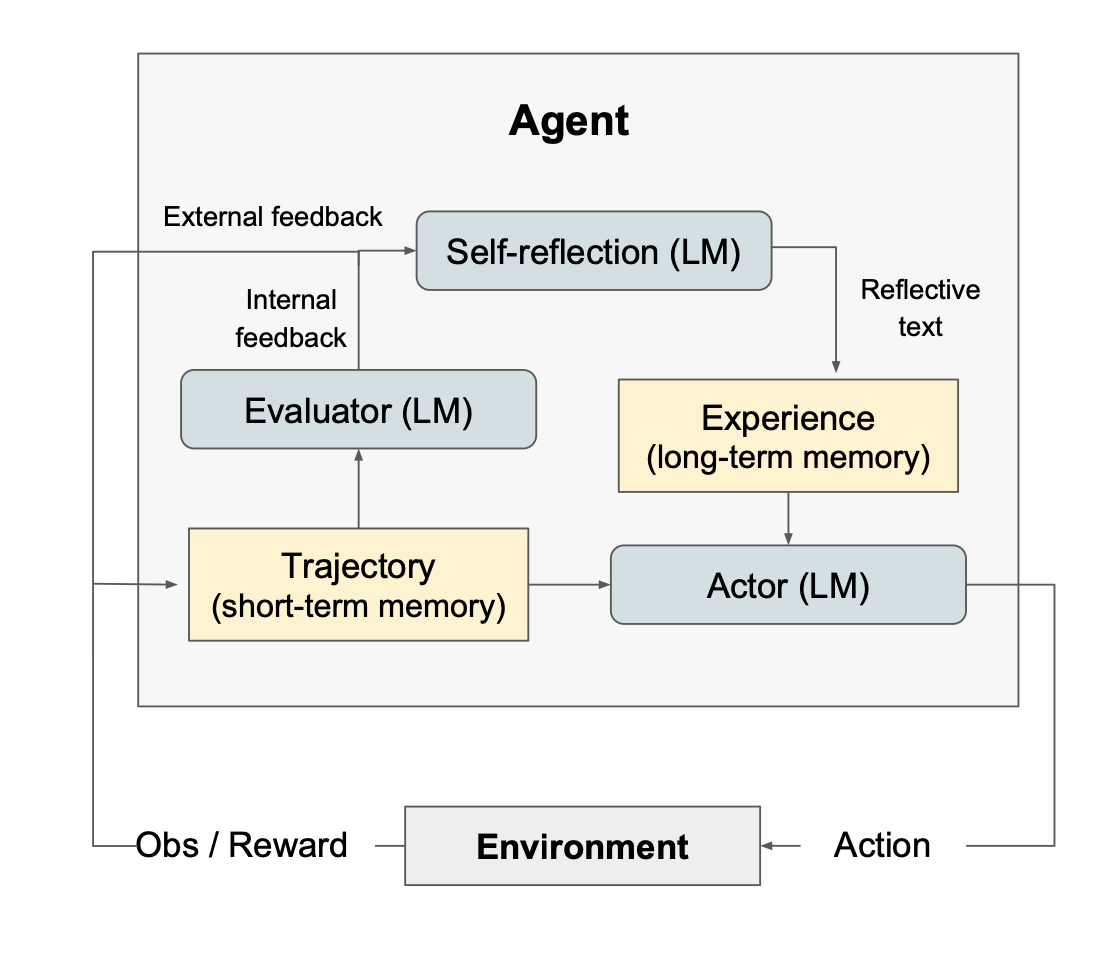
\includegraphics[width=8cm]{figures/reflexion3}
    \caption{Reflexion 的架构 \citep{shinn2024reflexion}，与强化学习的智能体/环境结构高度相似}\label{fig:reflexion2}
  \end{center}
\end{figure}
%  Figure~\ref{fig:reflexion} shows three different prompting applications. \begin{figure}   \begin{center}  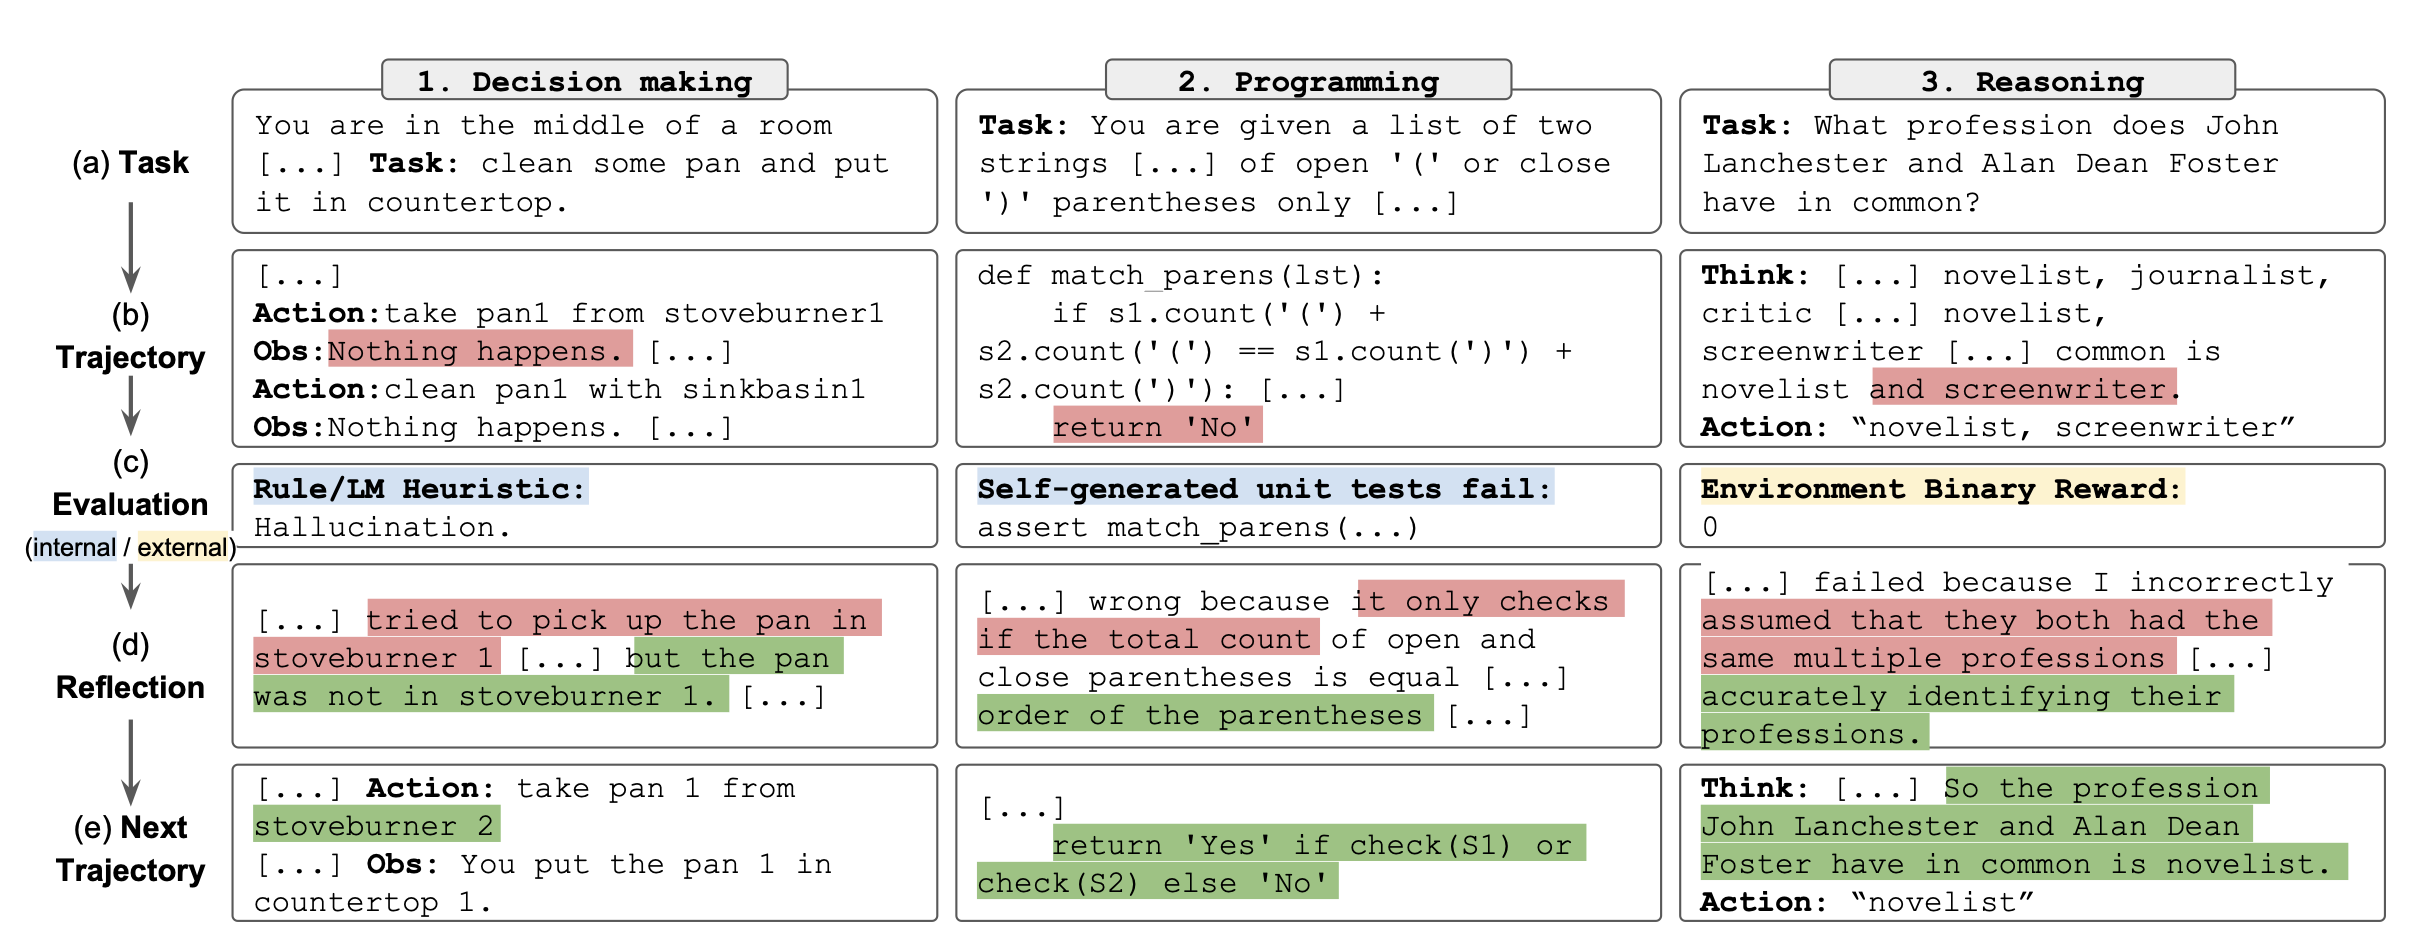
\includegraphics[width=12cm]{figures/reflexion} \caption{Comparison of three application areas  \citep{shinn2024reflexion}}\label{fig:reflexion} \end{center} \end{figure}

%\todo{Provide sequence of example prompts}
%A sequence of example prompts can be in the Game of 24. Reflexion first generates a position with the followin prompt: . It then loops through the possible answers, and evaluates the position with the prompt: . Then, it generates successor positions for each position, that are evaluated.
%\todo{Or do we want to do ReAct, is that simpler and more precise?}
%\todo{Or not, but describe Buffer of Thought?}

\paragraph{思维缓冲}
另一种方法是思维缓冲 \citep{yang2024buffer}，它朝元推理 \citep{gao2024meta} 迈出了一步。它引入一个元缓冲，用来存储高层的{\em 思维模板}。思维模板源自多种任务。思维缓冲用一个问题蒸馏器，把从不同问题中蒸馏出的高层
思维存入元缓冲，并对缓冲容量做主动管理。图~\ref{fig:bot2} 把思维缓冲与其他方法（如思维链与思维树）做了对比。思维缓冲在 24 点游戏（提升 11\%）与将杀（提升 51\%）等谜题上优于其他方法。
%
思维模板与元认知（对思考的思考）有关 \citep{didolkar2024metacognitive}。 
%
 \begin{figure}
   \begin{center}
     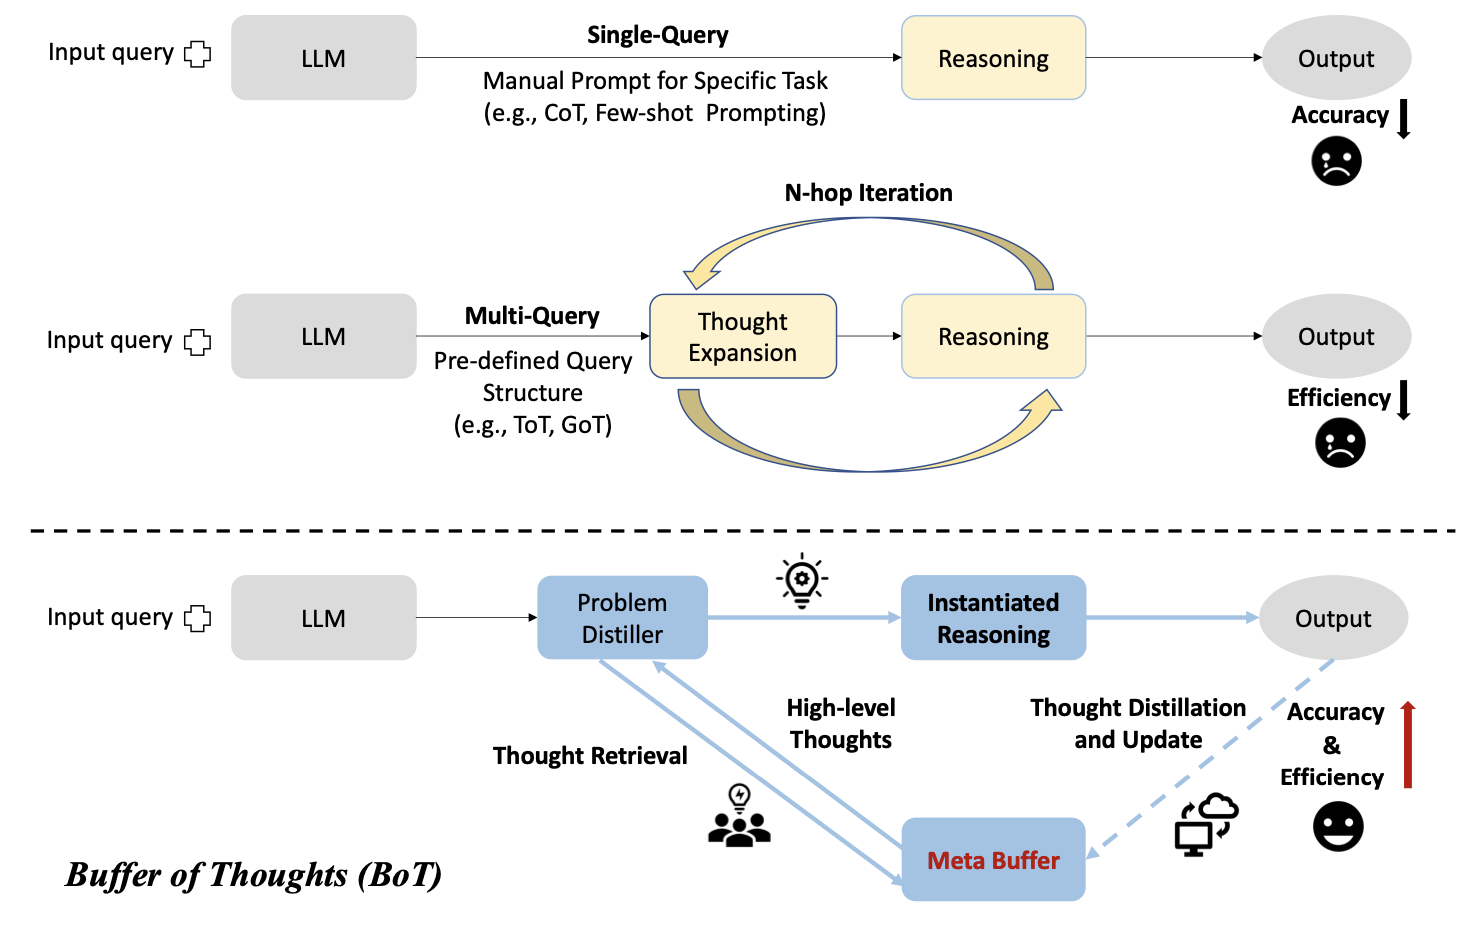
\includegraphics[width=10cm]{figures/bot}
     \caption{思维缓冲 \citep{yang2024buffer}}\label{fig:bot2}
   \end{center}
 \end{figure}

 



\paragraph{批评与提示词敏感性}
自我反思这一概念并非没有陷阱与批评。首先，「要求模型精炼自己的结果」这一基本想法本身就有疑问：为什么模型一开始不给出更好的答案？其次，\citet{huang2023large,shojaee2025illusion} 的研究发现某些研究存在方法学问题，例如使用了会泄露答案的数据标签、第二次精炼的提示词无意中比初始提示词透露了更多信息，以及在智能体与环境上使用同一个 LLM。在一项可复现性研究中，其表现并未超过思维链加自洽性 \citep{huang2023large}。LLM 对提示词中问题的表述方式很敏感。自我反思仍是一个年轻而活跃的研究领域，前提很吸引人，但开放问题很多。

我们介绍的这些方法可能会发起大量 LLM 调用，从而变得昂贵而缓慢。为你的问题找到最优方法，可能需要相当多的实验。在第~\ref{chap:balrog} 章中，我们将讨论一个实践案例研究，动手体验自我反思方法。请记住前面这些批评意见。


\subsubsection{可验证奖励强化学习}\label{sec:rlvr}
本章的重点是上下文学习。上下文学习发生在推理时，不训练也不改变任何参数。微调发生在训练时，确实会改变模型参数。不过在本节中，我们将简要谈谈微调与上下文学习的一种混合——我们会把训练与推理混在一起。

%We  do so because  algorithms have been developed that use inference time results for training purposes. 
%, interleaving inference and training.


可验证奖励强化学习指的是一种算法思路：在具有可验证结果的任务上训练
语言模型，例如数学解题与指令
遵循。尤其是对推理问题（如数学应用题与编程），人们发现推理时的思维链结果用于微调时能显著改进模型。

RLVR 是对基于人类反馈的强化学习（RLHF）的改进，它免除了对人类反馈的需求。在许多领域（如数学）中，存在一个简单函数就能检查答案是否正确，无需人类反馈。RLVR 沿用 RLHF 的目标，但把奖励模型换成了一个验证
函数。RLVR 在给定一组提示词时，从策略模型采样
补全结果，并用一个确定性函数验证其正确性。若正确，奖励为正，否则为 0。随后这个奖励被用于像 RLHF 那样，用 PPO \citep{schulman2017proximal}（一种标准的强化学习算法）来训练。


这类方法中一个有影响力的代表，是在 DeepSeek-R1 的开发中提出的 \cite{guo2025deepseek}。该方法与外部推理途径的区别在于，它强调模型自我生成的推理步骤。它通过强化学习来学习这些步骤，把数据生成与训练整合在同一个循环中。%This  approach holds significant potential for creating more autonomous and adaptive AI systems. 
由于降低了对监督数据的需求，
DeepSeek 的方法利用强化学习让模型% like DeepSeek-R1-Zero (the reasoning LLM before preference fine-tuning) 
自主地演化出推理技能。从一个基础模型出发并施加强化学习，系统便能识别并强化有效的推理模式。DeepSeek 使用组相对策略优化（GRPO），它%eliminates the need for a separate critic model by 
通过基于分组的打分来计算优势 \citep{shao2024deepseekmath}。%This approach allows the model to explore various problem-solving strategies and refine its thought processes without external inference-time control loops.

DeepSeek 方法的一个关键特征是：在微调过程中涌现出精巧的推理行为，例如反思与对备选解题方法的探索 \citep{mercer2025brief}。这些行为是模型与强化学习环境交互的结果而自发产生的，而非预先编程，也不需要外部的自我反思循环。例如，DeepSeek-R1-Zero 学会了通过重新审视最初的思路，为问题分配更多思考时间。
这种{\em 学会推理}的自主途径，可能带来更稳定、更具适应性的推理型 LLM。


%\todo{Add RLVR description}


GRPO 成功的原因之一，是它聚焦于存在可验证奖励的应用，从而使强化学习方法可用。对可验证奖励的关注相当成功，可验证奖励强化学习（RLVR）方法常被用于微调 LLM \citep{lambert2024tulu}。

%\todo{provide pseudocode example for RLVR finetunign setup? Is that already done in section 3.2.3?, nee verwijs naar TULU werk, die heel goede code heeft}


像 GRPO 这样的 RLVR 方法通常是动态使用的：用一次推理时的思维链查询来回答训练集中的一个问题，以此微调模型。也就是说，测试时的推理被用于微调。
%
DeepSeek 令人瞩目的成果 \citep{guo2025deepseek} 使 GRPO \citep{shao2024deepseekmath} 与 RLVR \citep{lambert2024tulu,guo2025deepseek,wen2025reinforcement,yue2025does} 成为极受欢迎的微调方法。

%Multi-step reasoning methods work well on planning problems where solutions can be quickly determined. The literature provides encouraging results in this domain.

%In the games of Chess and Hex encouraging results were achieved by pretrainging the decision transformer on minimax \citep{markeeva2024clrs,knuth1975analysis,plaat1996research} and MCTS \citep{browne2012survey} search traces \citep{schultz2024mastering,kempinski2025game}. Other works report encouraging results in the game of Othello \citep{li2023emergent,kempinski2025game,chen2025if}. 
%Algorithm of Thought achieved good results on decision making/reasoning tasks (Game of 24 and Mini Crosswords), both with finetuning and without finetuning (ICRL).

%Implicit reasoning is currently an active field of research, for results, see the literature \citep{li2025implicit}.


%\subsection{Implicit Reasoning}\label{sec:knowingdoing}
%Some studies pursue the concept of reasoning by LLMs further, and see how the current external control algorithms can be made internal. \citet{schultz2024mastering} showed how LLMs can be trained to do a tree search.
%\subsubsection{Pretraining on Decisions}
%The knowing-doing gap limits the capability of what single-prompt LLM approaches can achieve. Transformer architectures have been pretrained and finetuned for search \citep{schultz2024mastering}, reinforcement learning \citep{demircan2024sparse,schmied2025llms} and decision making \citep{lee2023context}. Research into implicit reasoning tries to find new network  architectures for multi-step reasoning \citep{li2025implicit}. Furthermore, for problems that require reasoning beyond a single sequence of reasoning steps, solutions have been introduced where the prompts are explicitly managed with external prompt-management algorithms, such as Tree of Thoughts \citep{yao2024tree} and ReAct \cite{yao2022react}.




%Implicit reasoning, inside LLM. Elegant, more efficient, black box
%\citep{li2025implicit}. Active field of research, many further developments to be expected. Reasoning power and efficiency will increase. Explicit prompt optimization allows more control of reasoning process. 
%\subsection{System 1 and System 2, Language and Combinatorics}
%Does this topic merit a full section? Maybe just a small observation is more appropriate? What is the point of this historical reflection?
%This is not a book about the history of AI.



\section{结语}
在前面的篇幅中，我们看到了语言模型的推理能力如何得以提升。最著名的方法是思维链，它是一种提示词工程方法，引导 LLM 在回答问题时给出多步推理，就像我们在学校里被示范如何解数学题那样。人们还引入了更精巧的提示词改进算法，从深度优先搜索，到自我反思，再到推理时强化学习方法。RLVR 之类的高级训练方法把推理结果与微调结合起来，取得了很强的训练效果。

\subsection{脆弱性}%\todo{Need another tone. Too cynical}
我们讨论了许多构造智能体运行框架的不同算法途径。之所以有这么多，原因有几方面。第一，智能体大语言模型领域还很年轻，存在许多挑战，因而催生了许多新解法。

第二，%This wealth of approaches might be quite enticing to try out yourself, to see your agent learn, reason, and self-reflect. By all means, go ahead! However, if you do so, chances are that your first attempt will not work. For example, the model will score unexpectedly low on the benchmark that you try. When you have found the problem, you will have learned a lot. Now  your second attempt seems to work, but you may find that it only does so with specific prompts, and does only self-reflect in very controlled circumstances: another cycle of learning for you to go through. 
这些方法相当脆弱。提示词上的微小改动，多一个或少一个逗号，有时就决定了方法能否奏效。超参数的微小变化，例如模型的温度，甚至换一个随机数种子，都可能带来很大影响。改变智能体运行框架的记忆管理方式，或换用另一个 LLM，也都可能对性能产生很大影响。

这或许让人感到不太满意。确实，这个领域还很年轻，方法要稳定下来还需要若干年。在你的实验中，请记住始终做多次运行——用不同的种子、不同的模型、不同的超参数设置。这会帮助你更好地理解你的方案在不同情境下如何工作。

%However, brittleness might be part of the reason why such a wealth of different approaches have been developed. They all work sometimes, in their own use cases, but not outside them, and  new approaches are invented. In a few years the field may have stabilized, we better understand when to use which approaches, and which to avoid. 
%At the moment, we are still in the wild-west phase of agentic LLM: results are brittle, many things are tried, some work, sometimes, and the field is propelled forward by the enthusiasm of new researchers. 
%Reasoning in LLMs is still an active field of research, and improvements are being published regularly. This is a young field, and when you try things, failure is to be expected. Be happy---failure is a learning opportunity.

\subsection{快思考与慢思考}
\label{sec:fast-and-slow}
作为本章的收尾，我们把 LLM 的推理放到一个更广阔的视角中讨论。在人工智能的历史上，可以看到两种途径或思想流派：符号主义 AI 与联结主义 AI。符号主义 AI 大致对应这样一种想法：智能最好建模为按照逻辑规则对符号进行操作。联结主义 AI 则研究智能是否会在相互连接的元素（无论是神经元、细胞、蚂蚁、人类还是机器人）之间的交互中自发涌现。符号主义 AI 汲取数学，联结主义 AI 汲取生物学。正如我们在第~\ref{sec:modernNLP} 节已看到的，两个流派都发展出了有用的方法，也都取得过重要成功（例如搜索算法与推理，或深度学习与 LLM）。

%From psychology comes a book that introduces the concepts of thinking slow and thinking fast. 
2011 年，Daniel Kahneman 出版了{\em 《思考，快与慢》}一书，%Much of the terminology of this field is
%inspired by the System 1 and System 2 distinction that is popularized
%by
其中用系统~1 与系统~2
这两个术语把人类思维区分为直觉式的快思考与
审慎式的慢思考 \citep{kahneman2011thinking}。这些术语在
人工智能中变得流行，快思考被联系到联想式查找，慢思考被联系到多步推理。在推理时，零样本 LLM 进行的是快思考（系统 1 思考）。
推理时的分步方法（无论是通过更长的提示词，还是借助智能体运行框架）执行的是审慎的
慢思考
（系统 2 思考）。%As we will see, System 2 approaches achieve better performance on reasoning tasks \citep{plaat2024reasoning}.
%As we will see, agent-based learning
%methods are used to improve reasoning performance of LLMs. The agent
%methods are still used to improve LLM performance (Section~\ref{sec:action}
%uses LLMs to improve agent actions).

LLM 基于联结主义 AI 传统（系统 1）。在推理时
使用工具，为 LLM 这部分增强了来自符号主义 AI 传统的
知识检索或处理工具（系统 2）。

我们应当注意：尽管研究者有时会把 LLM 及其能力拟人化，但 LLM 只做下一个词元预测。LLM 离人类还差得很远。通过生成更多词元来构成答案（逐步推理），从提示词到最终答案的词元路径变长了。这之所以更常导向正确答案，可能是因为它朝答案方向迈出了更小的步子，使正确答案在每一步之间都变得更可信——而不是因为它类似于人类被教导的解题方式。推理是在收窄概率分布，使正确答案更可能被生成，这与人类认知层面的解释无关 \citep{guo2025deepseek}。

\subsection{小结}
在本章中，我们讨论了 LLM 如何通过下一个词元预测解决语言任务，以及如何解决需要多步推理的任务。我们讨论了管理复杂推理结构的各种方式。
%, mostly using  explicit prompt management based on reinforcement learning.

大多数方法%that we discussed in this chapter 
都是上下文方法，高效且易用，因为引导推理的提示词是用户可读的。我们引入了智能体运行框架这一角色，用于改进提示词与管理记忆。我们还触及了一些使用预训练与微调的方法，它们不只针对语言部分，也用于整合多步推理。这些方法由此训练出能进行决策的模型，超越了语言模型中的纯下一个词元预测。%Transformers are theoretically Turing-complete computation architectures, that are able to perform tasks beyond language. 

在构建这类更丰富的模型方面已有大量工作，它们加入视觉推理、决策与行动，成为 LLM 不可分割的一部分。在下一章中，我们将更深入地考察这些经过预训练与微调的多模态模型。

\bibliographystyle{plainnat}
\bibliography{agenticbook,refs,case,synthetic}
